\documentclass[utf8,aspectratio=169,ngerman,english,usenames,dvipsnames]{beamer}
\usetheme[darkmode,fancyfonts,totalframenumber,mathastext,TNF,noimprint]{jku}

\usepackage{tikzpagenodes}
\usetikzlibrary{calc}
\tikzset{frameoverlay/.style={overlay,remember picture,shift={(current page text area.south west)},
x={($(current page text area.south east)-(current page text area.south west)$)},
y={($(current page text area.north west)-(current page text area.south west)$)},nodes={anchor=south west}}}

\usepackage{booktabs}
\usepackage{tabularx}
\usepackage{tcolorbox}
\usepackage{wasysym}
\usepackage{pifont}
\usepackage{listings}
\usepackage{multicol}
\usepackage{tabularray}
\usepackage{caption}
\usepackage[absolute,overlay]{textpos}
\captionsetup{skip=0pt}
\newcommand{\cmark}{\ding{51}}
\newcommand{\xmark}{\ding{55}}
\newcommand{\rarr}{\ding{212}}
\newcommand{\larr}{\raisebox{\depth}{\rotatebox{180}{\rarr}}}
\usepackage{csquotes}
\usepackage[backend=biber,citestyle=authoryear,sortcites=true,style=ACM-Reference-Format]{biblatex}

\graphicspath{ {../../graphics/} }

%%%%%%%%%%%%%%%%%%%%%%%%%%%%%%%%%%%%%%%%%%%%%%%%%%%%%%%%%%%%%%%%%%%%%%%%%%%%%%%%%%%%%%%%%%%%%%%%%%%%%
%%%%%%%%%%%%%%%%%%%%%%%%%%%%%%%%%%%%%%%%%%%%%%%%%%%%%%%%%%%%%%%%%%%%%%%%%%%%%%%%%%%%%%%%%%%%%%%%%%%%%
\begin{document}

\title{CLOOB: Modern Hopfield Networks with InfoLOOB Outperform CLIP}
\subtitle{Seminar in AI}
\author{Pascal Pilz}
\institute{Institute for Machine Learning}
\date[\today]{} % use this to set the date except for the title page (effectively in the footer only)

\maketitle

%%%%%%%%%%%%%%%%%%%%%%%%%%%%%%%%%%%%%%%%%%%%%%%%%%%%%%%%%%%%%%%%%%%%%%%%%%%%%%%%%%%%%%%%%%%%%%%%%%%%%
\section{Motivation and Setup}
    
\begin{frame}{Contrastive Learning and Zero-shot Transfer Learning}
    \pause
    \begin{columns}
        \begin{column}{0.375\textwidth}
            \textbf{Contrastive Learning:}
            \begin{itemize}
                \item self-supervised technique
            \end{itemize}
            \begin{figure}
                \centering
                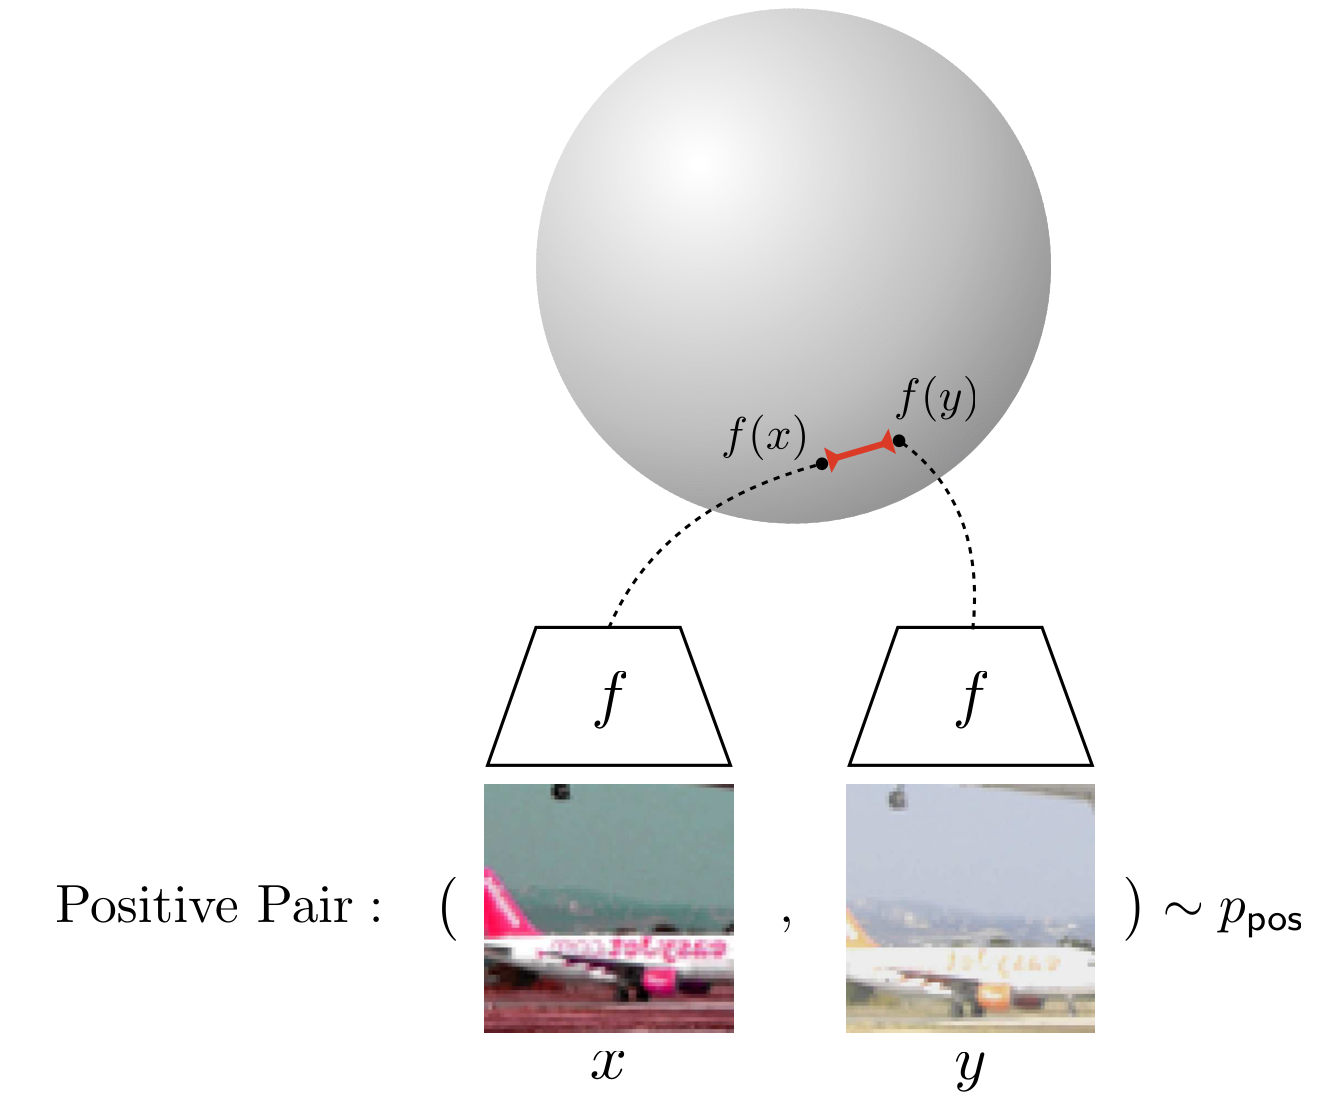
\includegraphics[width=1.0\textwidth]{sphere}
            \end{figure}
        \end{column}
        \pause
        \begin{column}{0.625\textwidth}
            \textbf{Zero-shot Transfer Learning:}
            \begin{itemize}
                \item model needs to generalize well
            \end{itemize}
            \begin{figure}
                \centering
                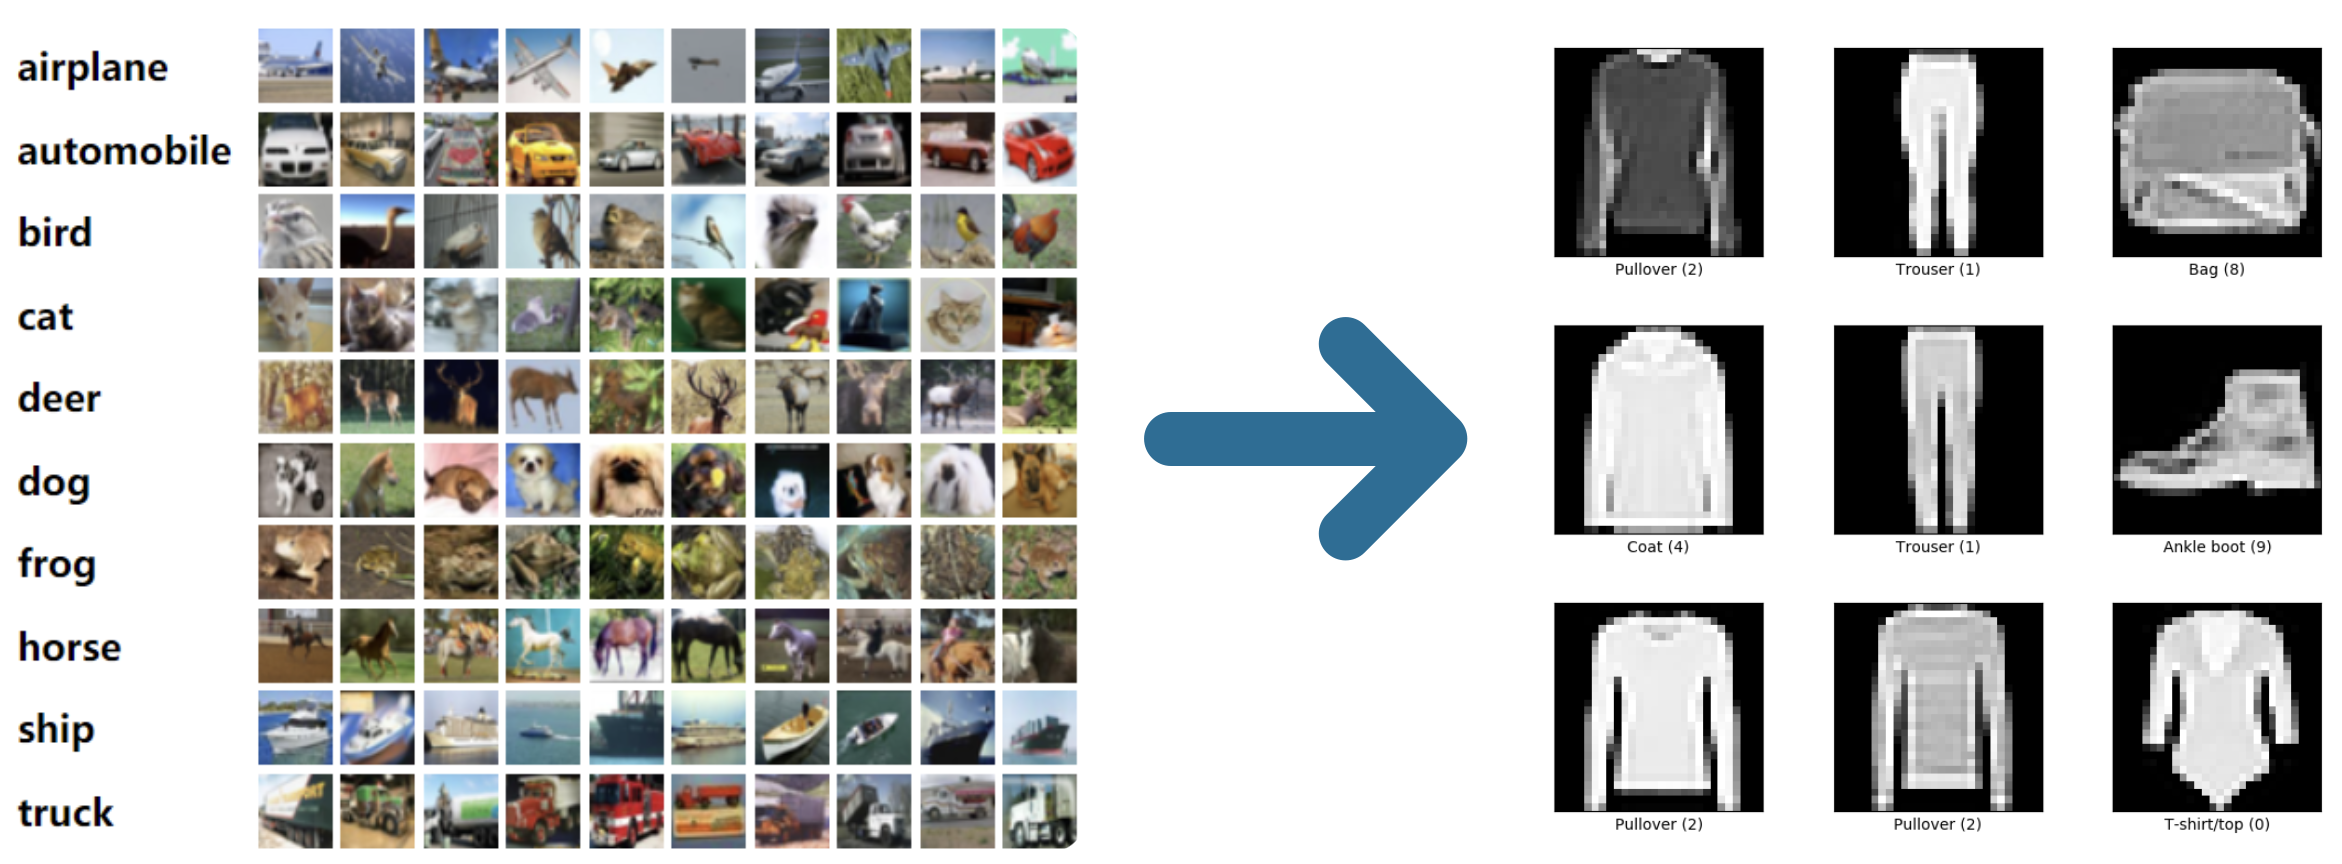
\includegraphics[width=0.9\textwidth]{transfer_learning}
            \end{figure}
        \end{column}
    \end{columns}
\end{frame}

\begin{frame}{CLIP (Contrastive Language-Image Pretraining) by OpenAI}
    \pause
    \begin{figure}
        \centering
        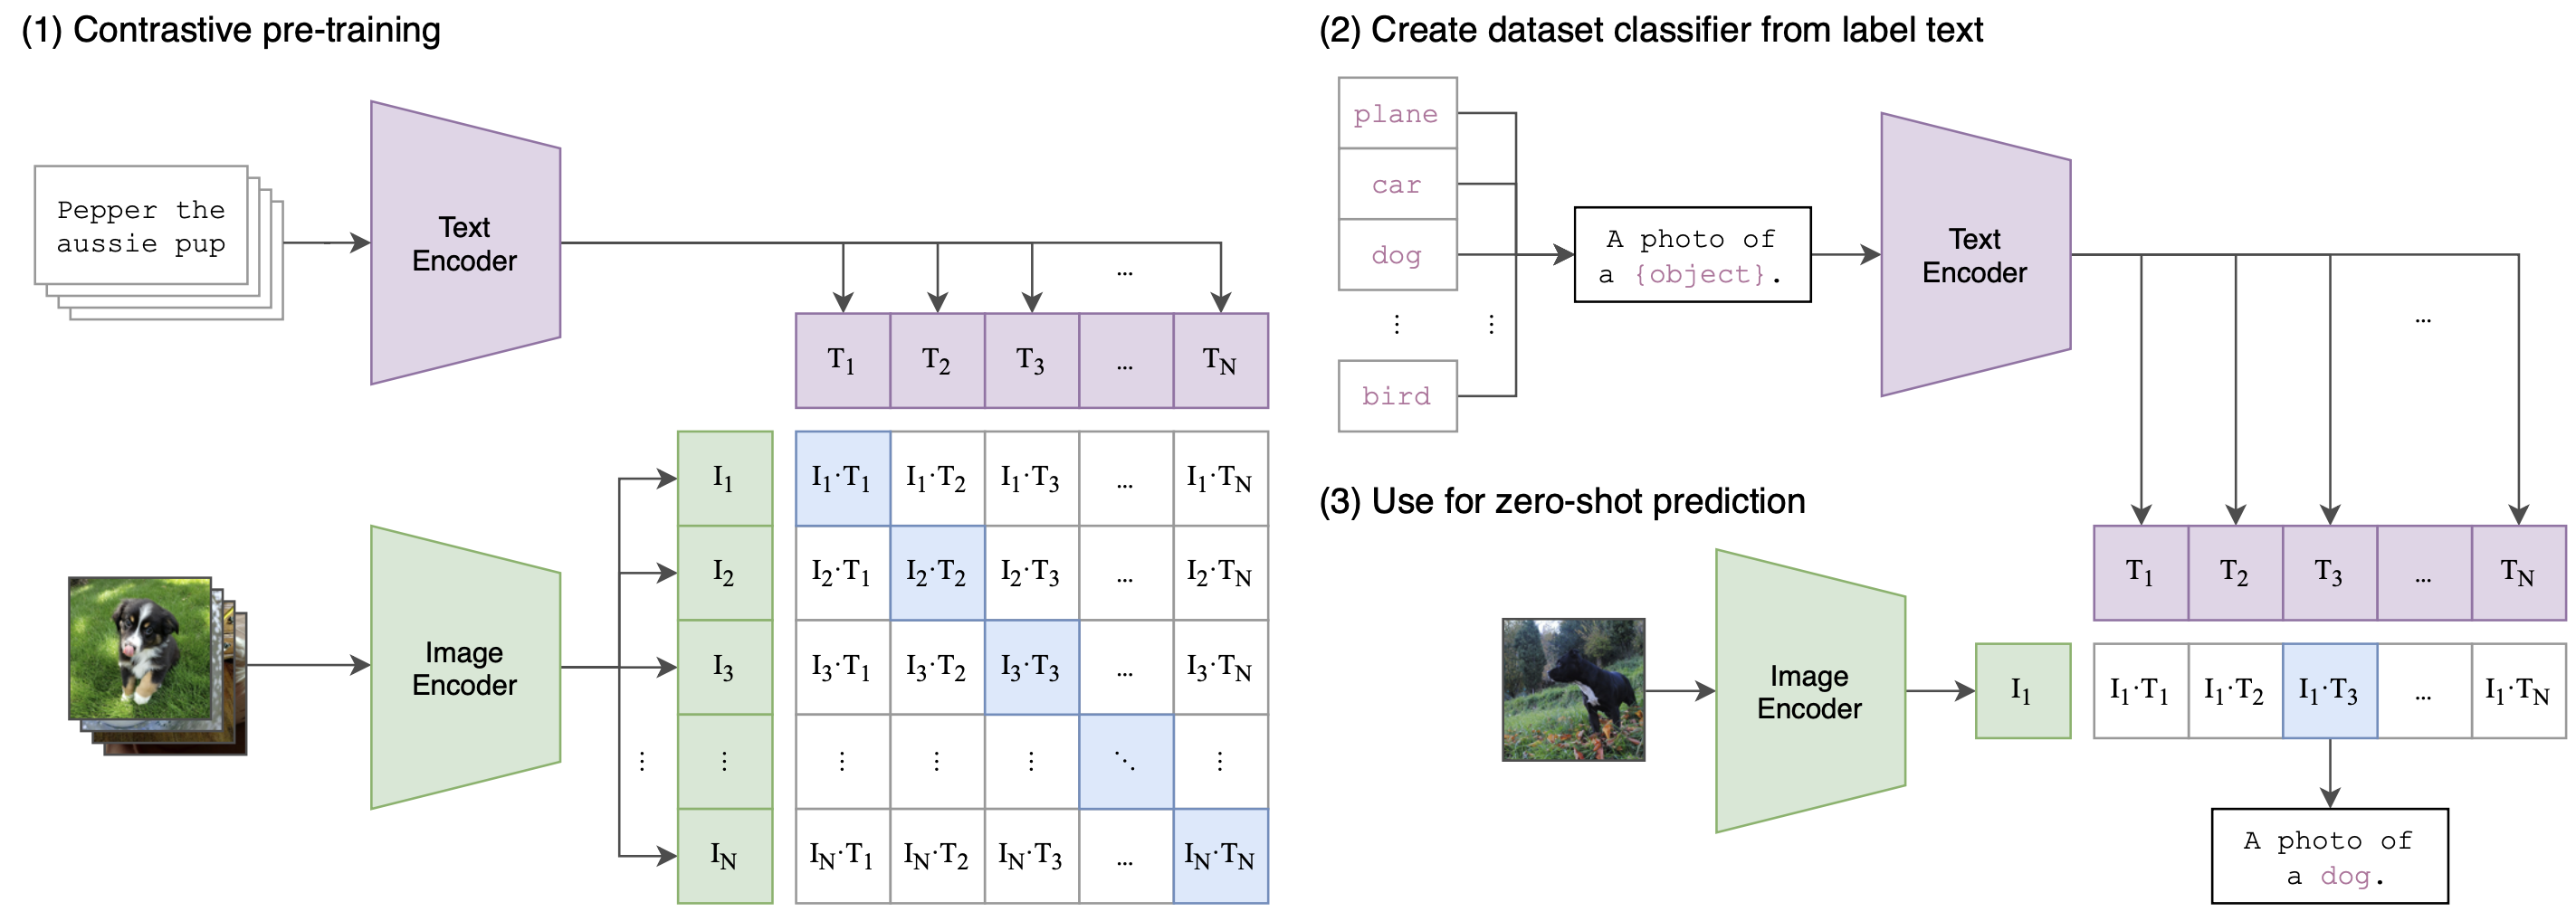
\includegraphics[width=1.0\textwidth]{CLIP_architecture}
    \end{figure}
    \pause
    \vspace*{-28ex}
    \begin{center}
        \rotatebox{20}
        {\begin{tcolorbox}[colback=white, colframe=black, enlarge top by=2mm, enlarge bottom by=2mm, width=0.65\linewidth]
            {\textcolor{red}{\Huge \textbf{EXPLAINING AWAY}}}
        \end{tcolorbox}}
    \end{center}
\end{frame}

\begin{frame}{Explaining Away --- Co-occurrences and Covariance structure}
    \pause
    \begin{tikzpicture}
        \node[anchor=south west, inner sep=0] (image) at (0,1) {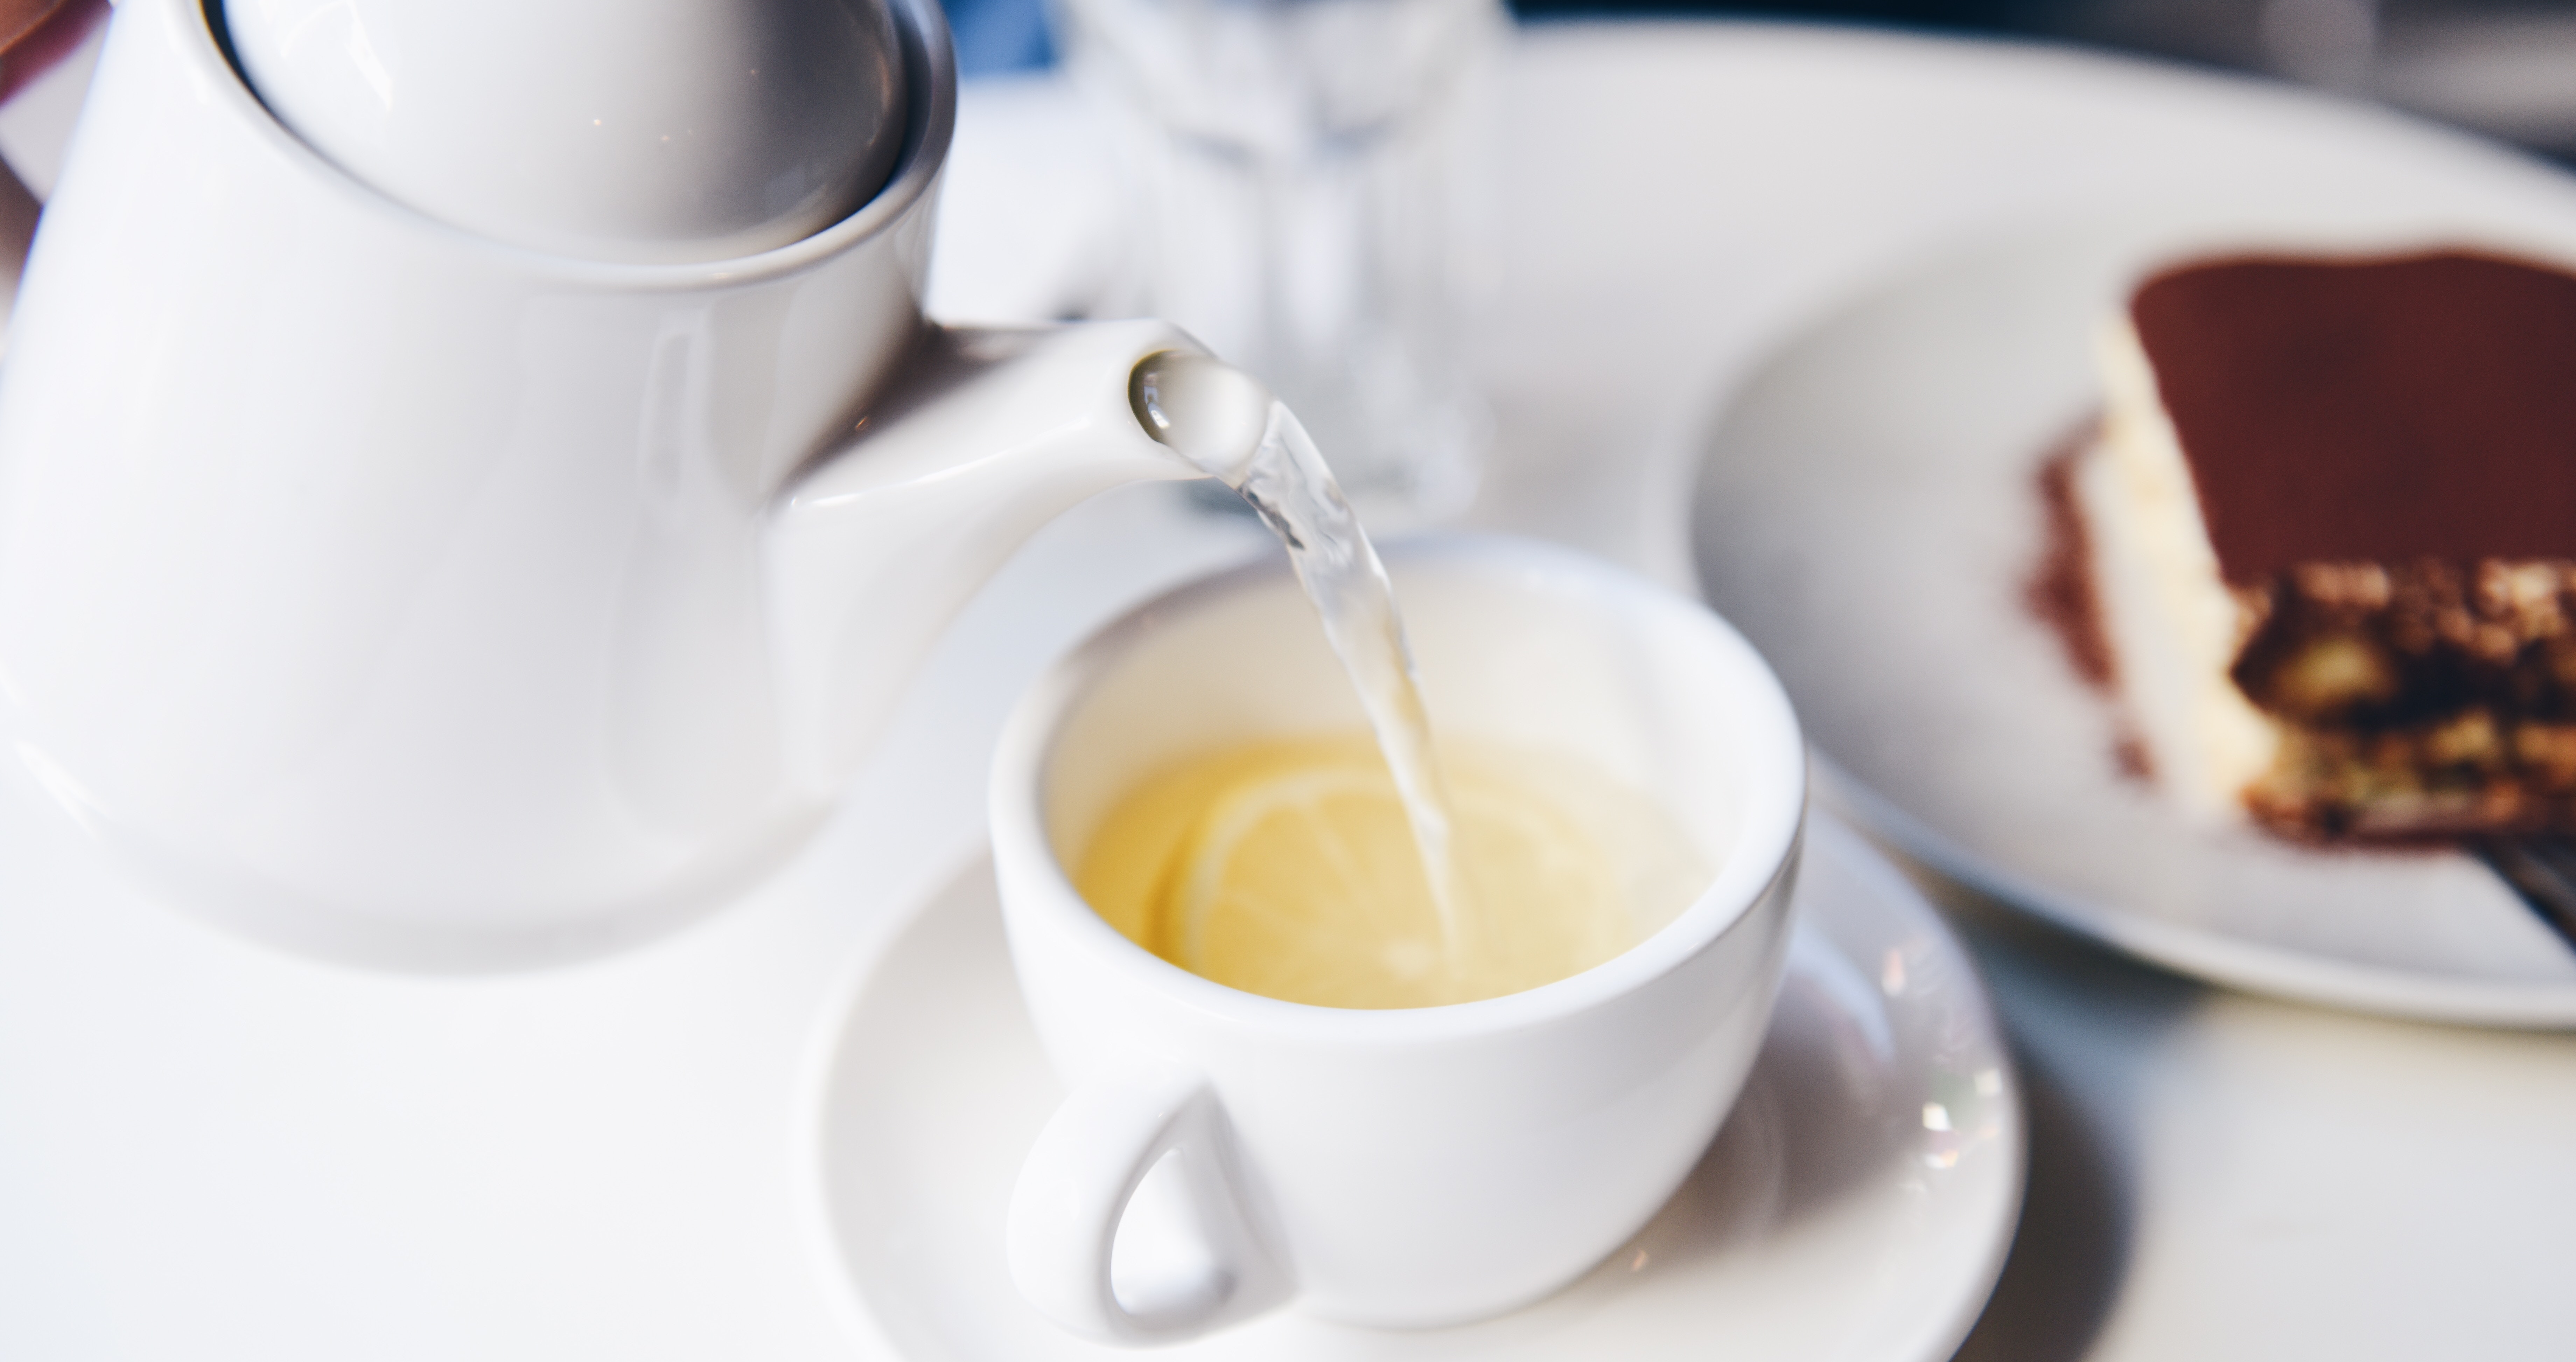
\includegraphics[width=0.625\textwidth] {teahouse_real}};
        \begin{scope}[shift={(image.south west)}, x={(image.south east)}, y={(image.north west)}]
            \filldraw<2>[white, even odd rule] (0,0) rectangle (1,1) (0.9, 0.6) circle (1.3cm);
            \filldraw<3->[opacity=0, even odd rule] (0,0) rectangle (1,1);
        \end{scope}
        \node<4>[anchor=south west, inner sep=0] (image) at (5,0) {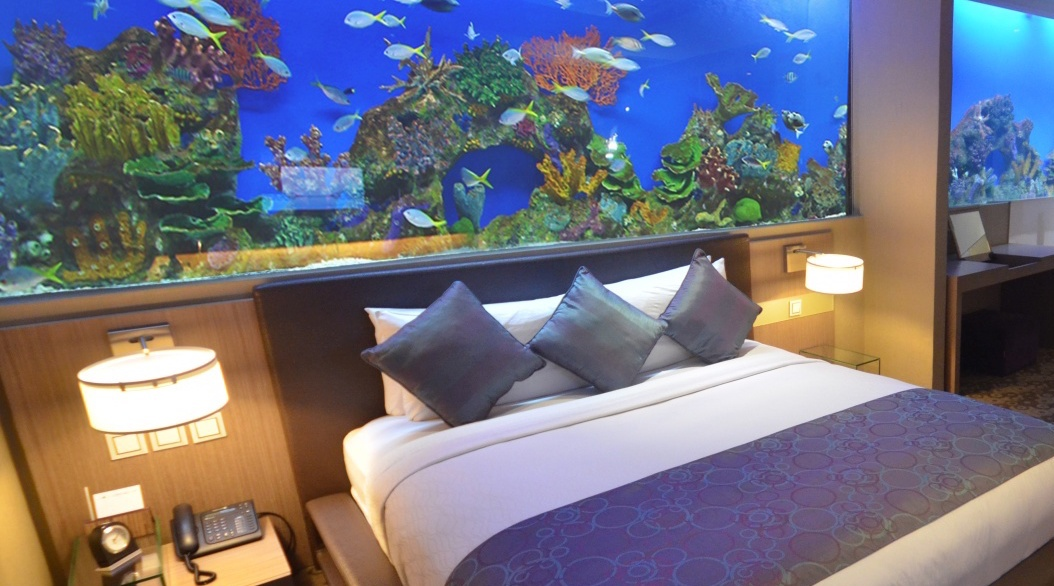
\includegraphics[width=0.625\textwidth] {bedroom_aquarium}};
    \end{tikzpicture}
\end{frame}

%%%%%%%%%%%%%%%%%%%%%%%%%%%%%%%%%%%%%%%%%%%%%%%%%%%%%%%%%%%%%%%%%%%%%%%%%%%%%%%%%%%%%%%%%%%%%%%%%%%%%
\section{Modern Hopfield Networks}

\begin{frame}{Excursus: Modern Hopfield Networks}
    \pause
    \begin{figure}
        \centering
        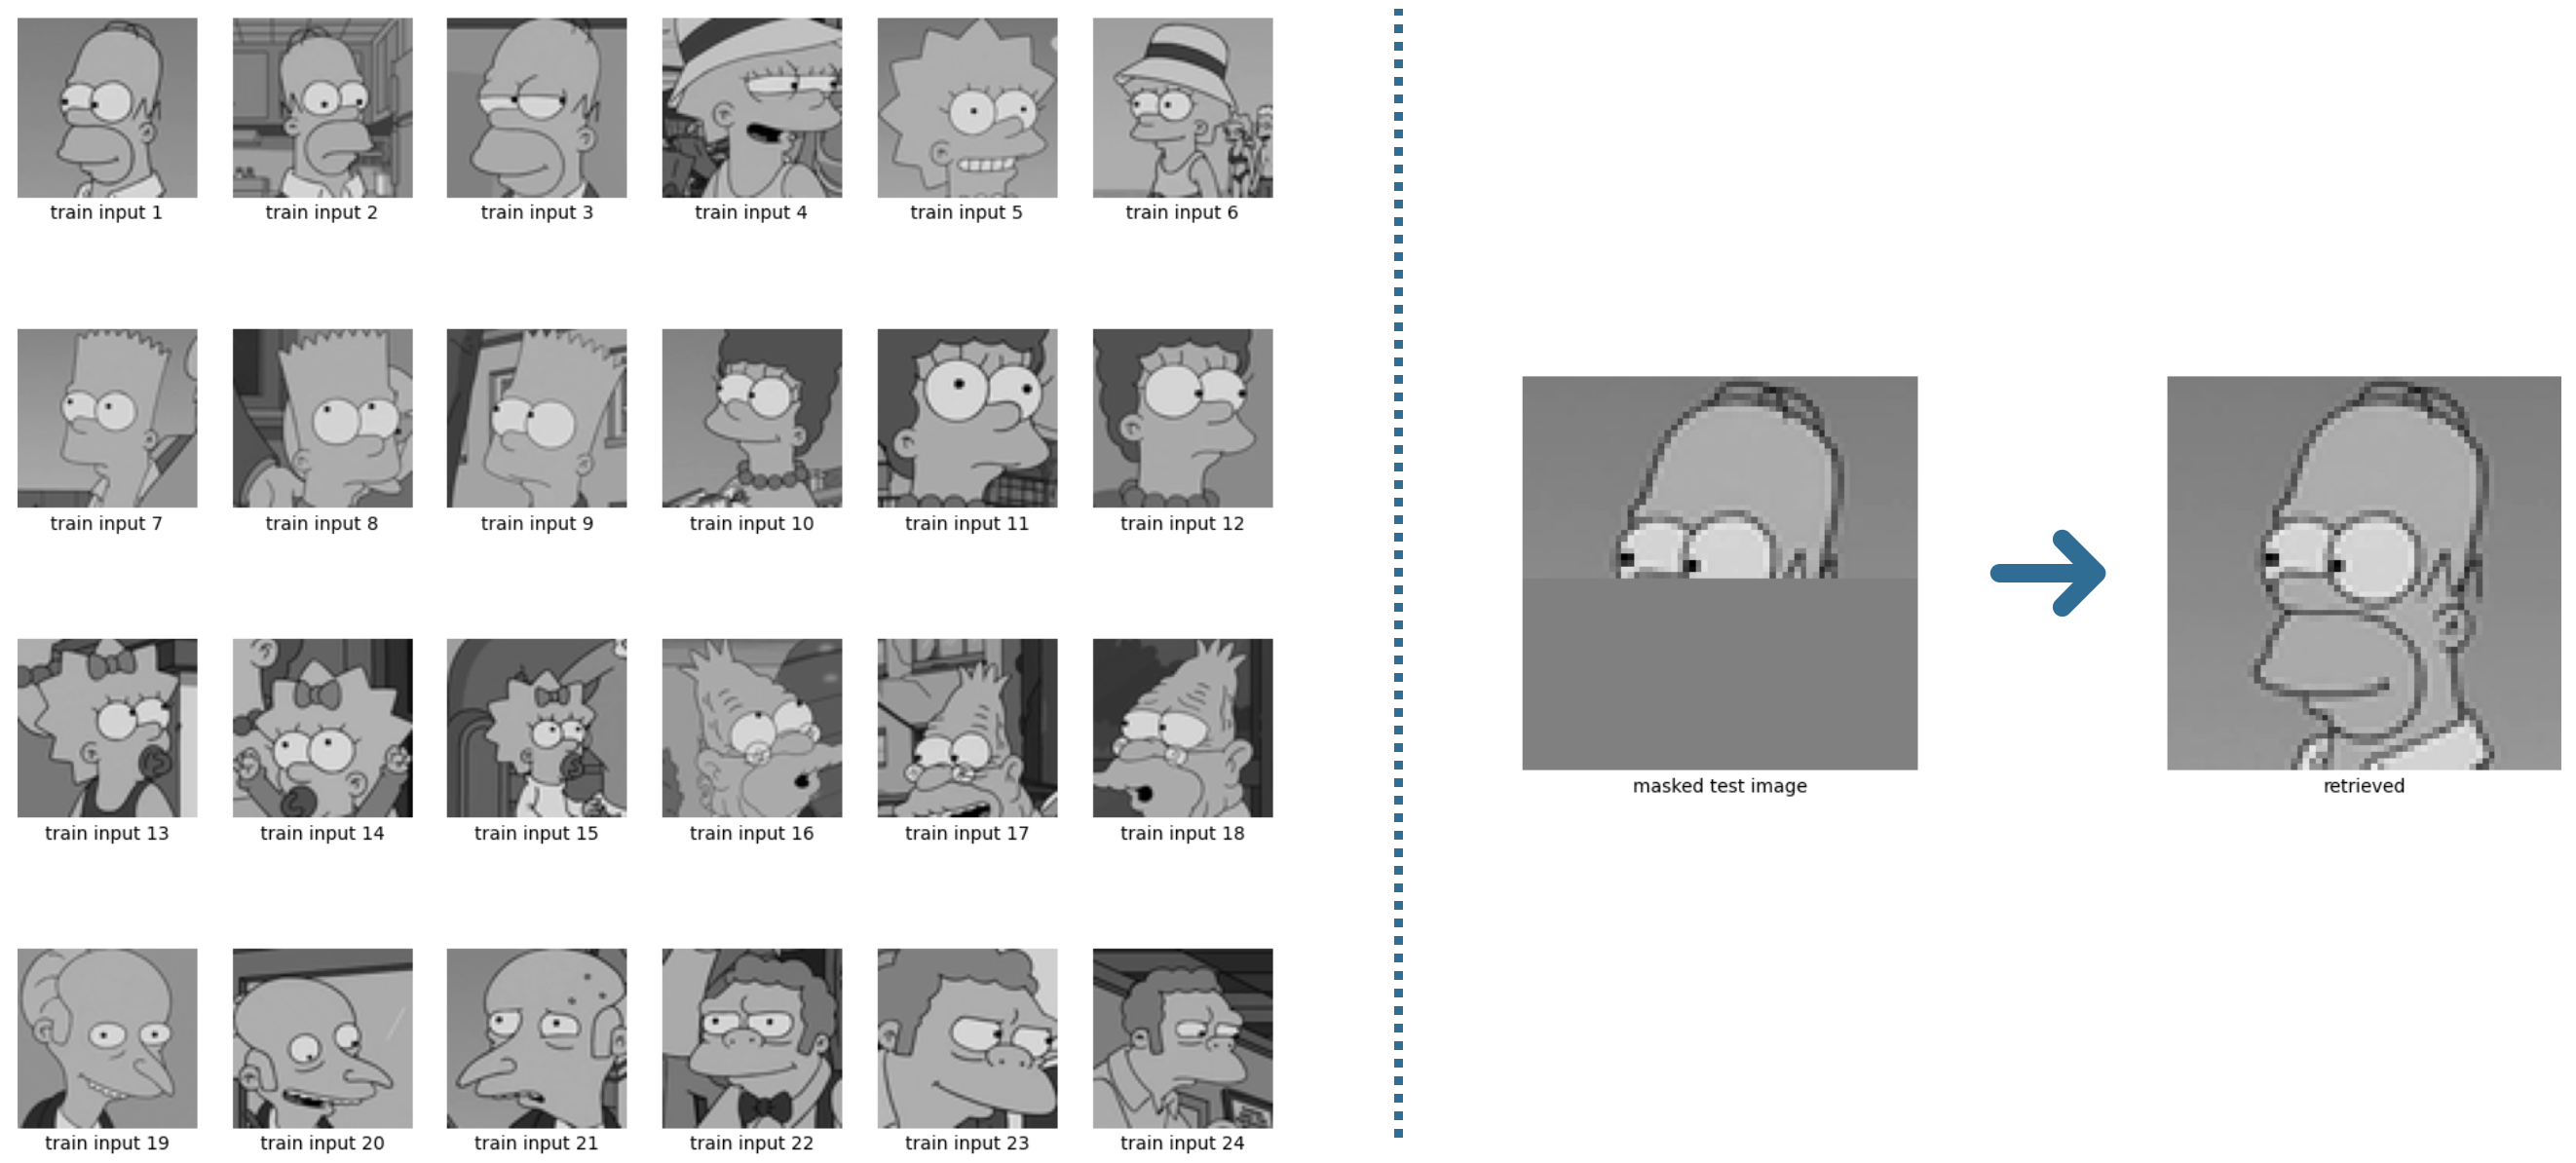
\includegraphics[width=0.8\textwidth]{MHN_homer}
    \end{figure}
\end{frame}

\begin{frame}{Amplifying Co-occurrences and Covariance Structures}
    \begin{tikzpicture}
        \node<2->[anchor=south west, inner sep=0] (image) at (0,1) {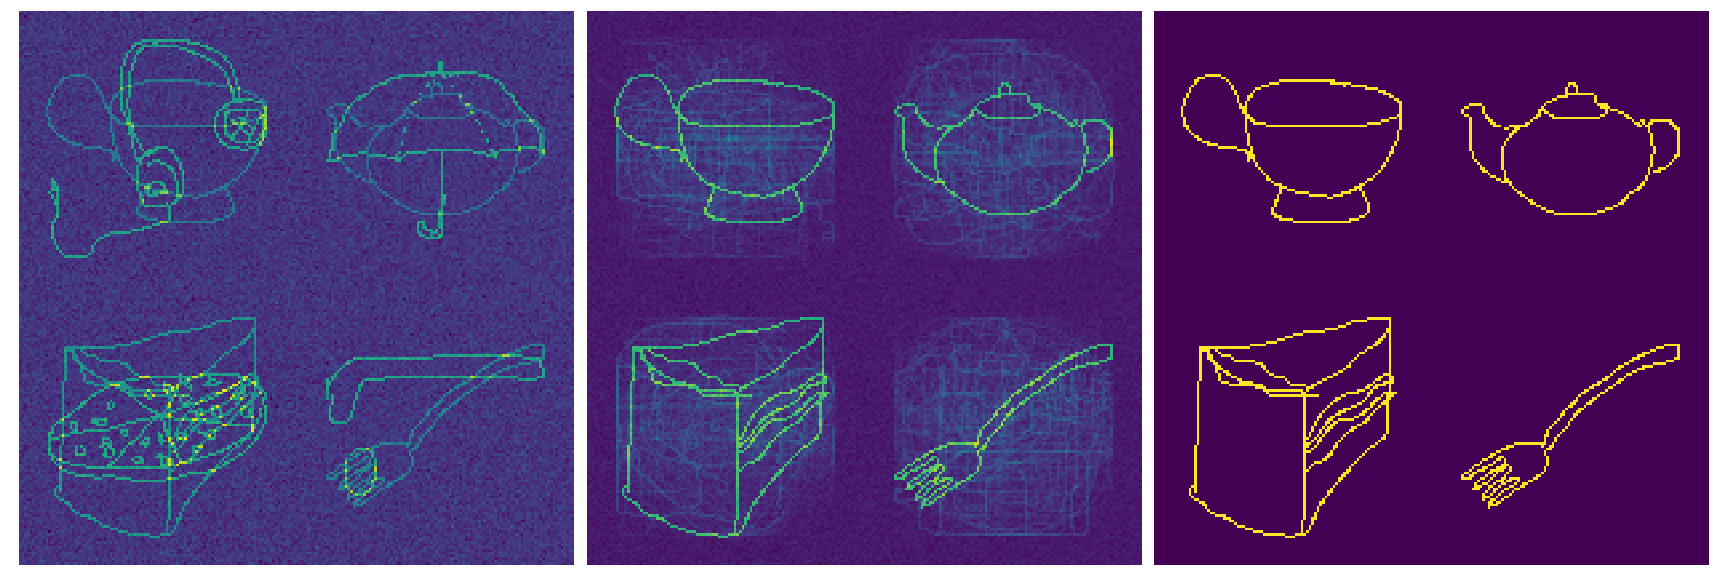
\includegraphics[width=0.7\textwidth] {sketch_tea_hopfield}};
        \node<3->[anchor=south west, inner sep=0] (image) at (4.3,-1) {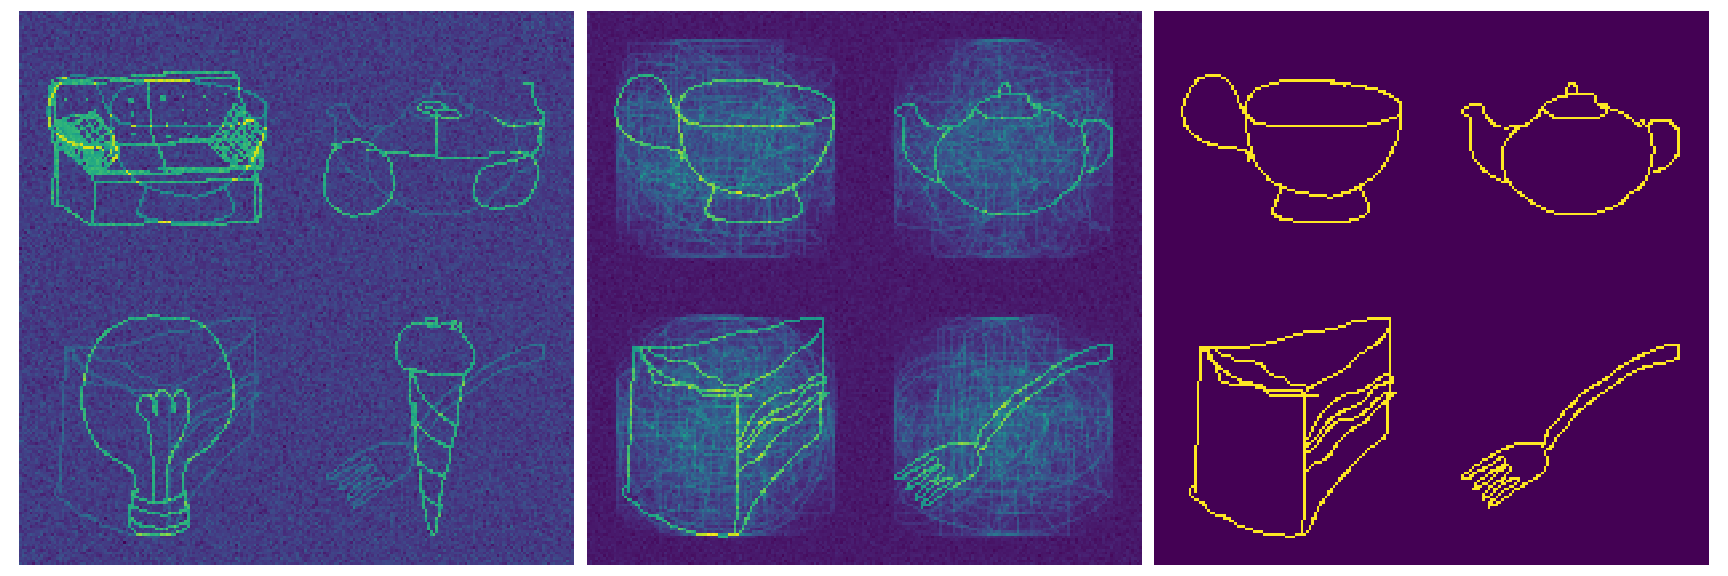
\includegraphics[width=0.7\textwidth] {sketch_tea2_hopfield}};
    \end{tikzpicture}
\end{frame}

\begin{frame}{CLOOB Architecture}
    \pause
    \begin{figure}
        \centering
        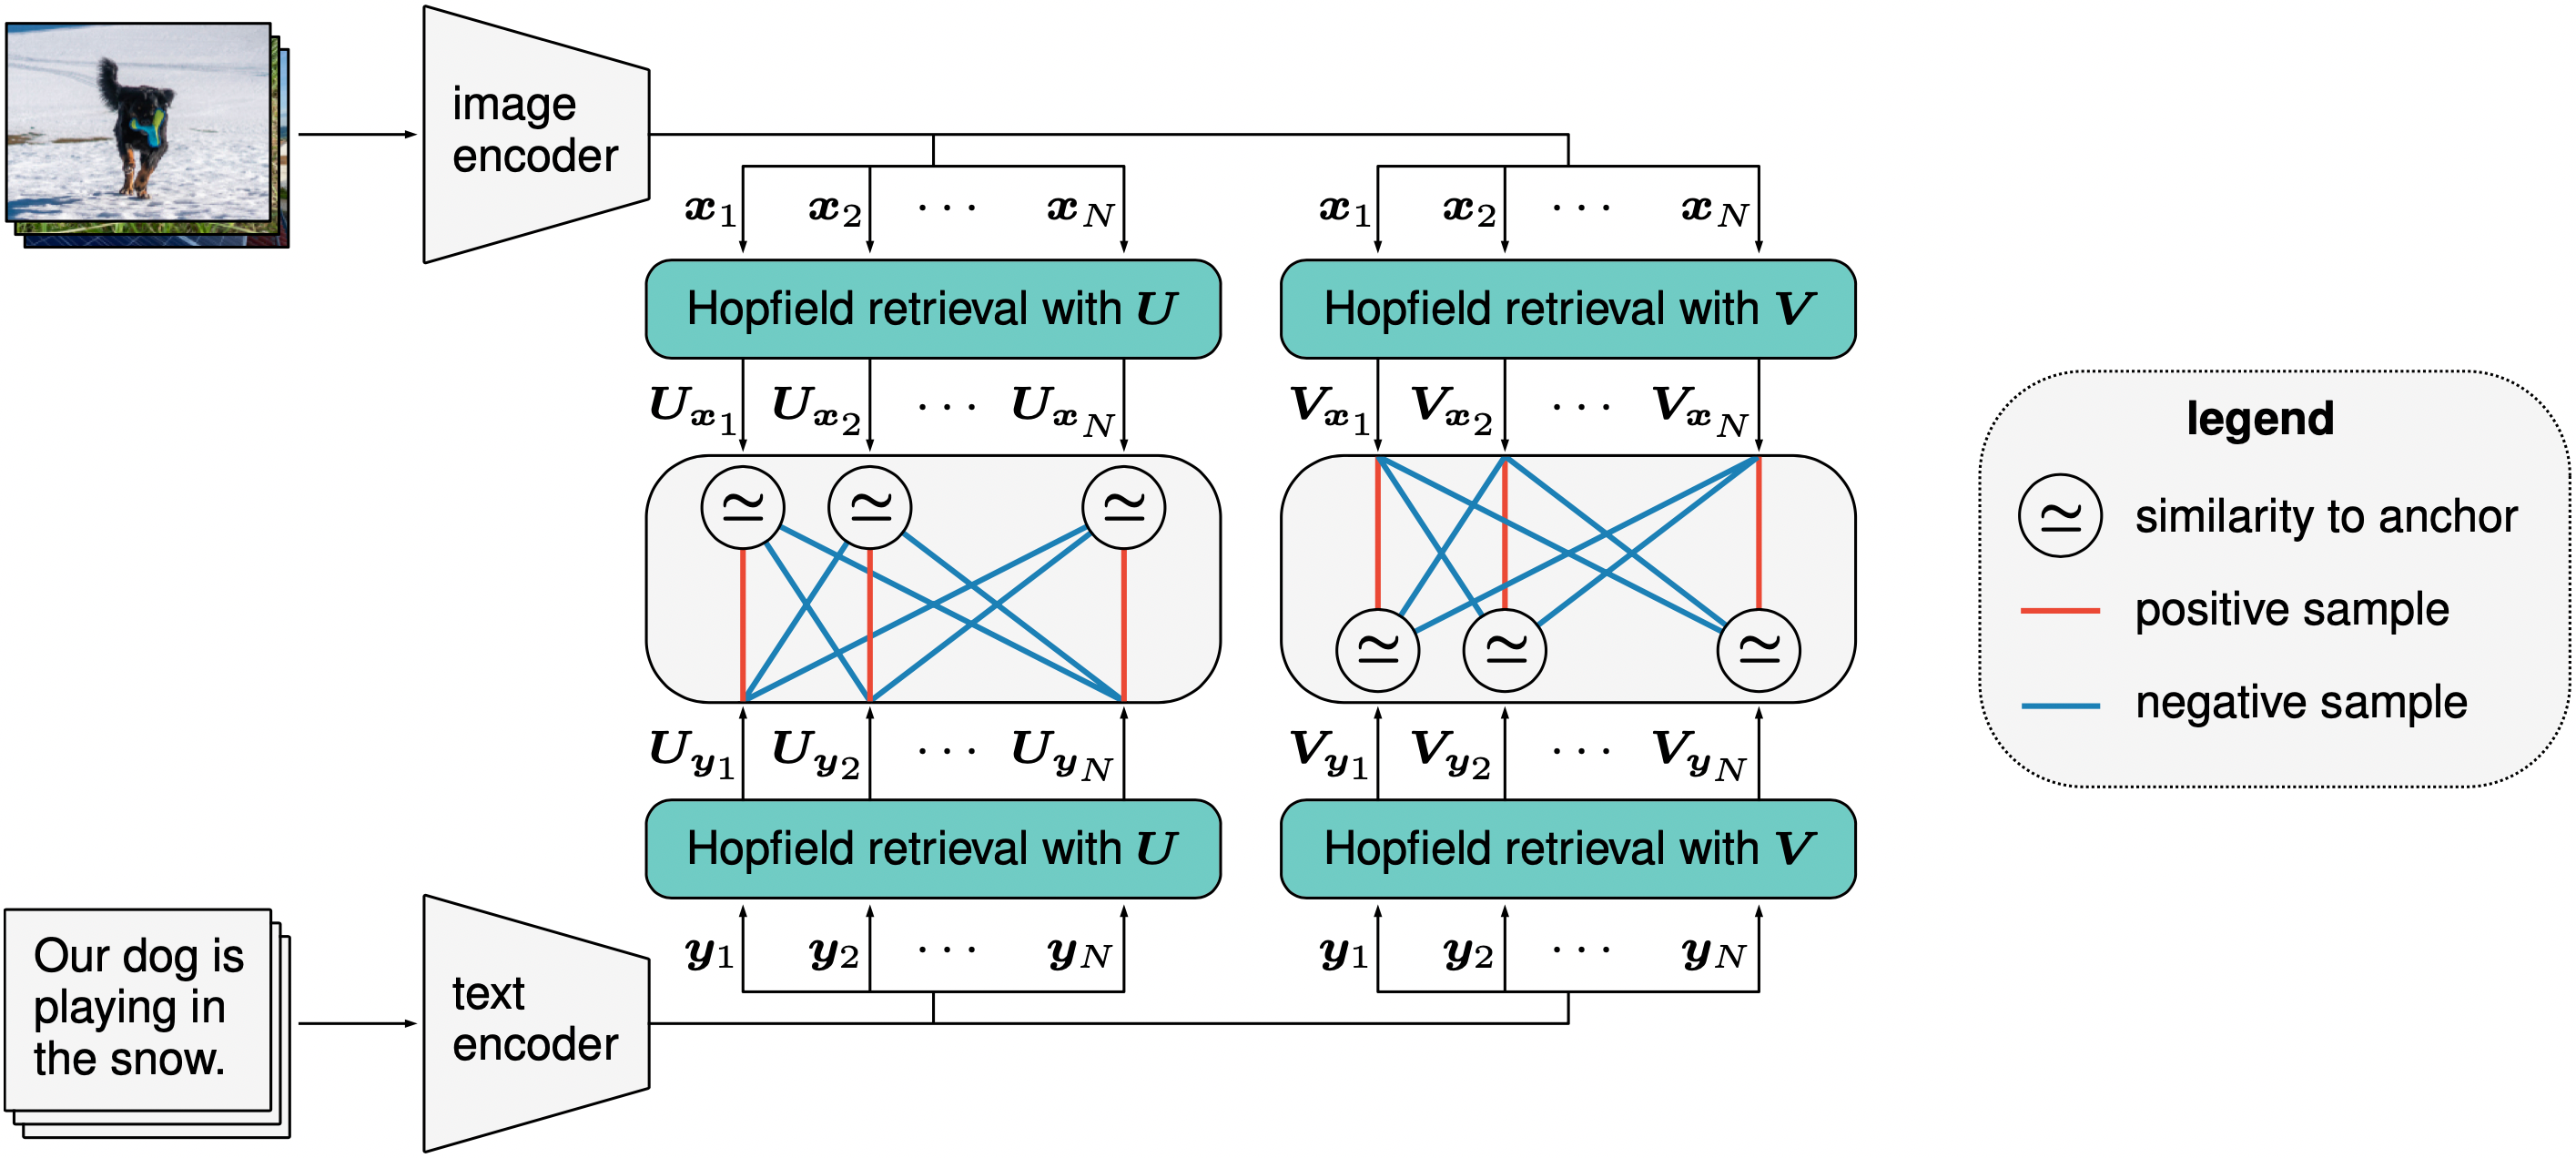
\includegraphics[width=0.8\textwidth]{CLOOB_architecture}
    \end{figure}
    \pause
    \vspace*{-28ex}
    \begin{center}
        \rotatebox{20}
        {\begin{tcolorbox}[colback=white, colframe=black, enlarge top by=2mm, enlarge bottom by=2mm, width=0.8\linewidth]
            {\textcolor{red}{\Huge \textbf{SATURATION PROBLEM}}}
        \end{tcolorbox}}
    \end{center}
\end{frame}

%%%%%%%%%%%%%%%%%%%%%%%%%%%%%%%%%%%%%%%%%%%%%%%%%%%%%%%%%%%%%%%%%%%%%%%%%%%%%%%%%%%%%%%%%%%%%%%%%%%%%
\section{InfoNCE, InfoLOOB, and CLOOB}

\begin{frame}{InfoNCE (Noise Contrastive Estimation) --- CLIP's Objective}
    \begin{onlyenv}<2>
        \begin{equation*}
            \operatorname{L_{InfoNCE}} =
            - \frac{1}{N} \ln \sum_{i=1}^{N} \frac{\exp(\tau^{-1} \mathbf{x}_i^T \mathbf{y}_i)}{\sum_{j=1}^{N} \exp(\tau^{-1} \mathbf{x}_i^T \mathbf{y}_j)}
            - \frac{1}{N} \sum_{i=1}^{N} \ln \frac{\exp(\tau^{-1} \mathbf{x}_i^T \mathbf{y}_i)}{\sum_{j=1}^{N} \exp(\tau^{-1} \mathbf{x}_j^T \mathbf{y}_i)}
        \end{equation*}
    \end{onlyenv}

    \begin{onlyenv}<3>
        \begin{equation*}
            \operatorname{L_{InfoNCE}} =
            - \frac{1}{N} \ln \sum_{i=1}^{N} \frac{\exp(\tau^{-1} \mathbf{\textcolor{red}{x}}_i^T \mathbf{\textcolor{blue}{y}}_i)}{\sum_{j=1}^{N} \exp(\tau^{-1} \mathbf{\textcolor{red}{x}}_i^T \mathbf{\textcolor{blue}{y}}_j)}
            - \frac{1}{N} \sum_{i=1}^{N} \ln \frac{\exp(\tau^{-1} \mathbf{\textcolor{red}{x}}_i^T \mathbf{\textcolor{blue}{y}}_i)}{\sum_{j=1}^{N} \exp(\tau^{-1} \mathbf{\textcolor{red}{x}}_j^T \mathbf{\textcolor{blue}{y}}_i)}
        \end{equation*}
        \begin{columns}
            \begin{column}{0.5\textwidth}
                \begin{itemize}
                    \item $\mathbf{\textcolor{red}{x}}_i$ --- \textcolor{red}{image} embedding
                    \item $\mathbf{\textcolor{blue}{y}}_i$ --- \textcolor{blue}{text} embedding
                \end{itemize}
            \end{column}
            \begin{column}{0.5\textwidth}
                \begin{figure}
                    \centering
                    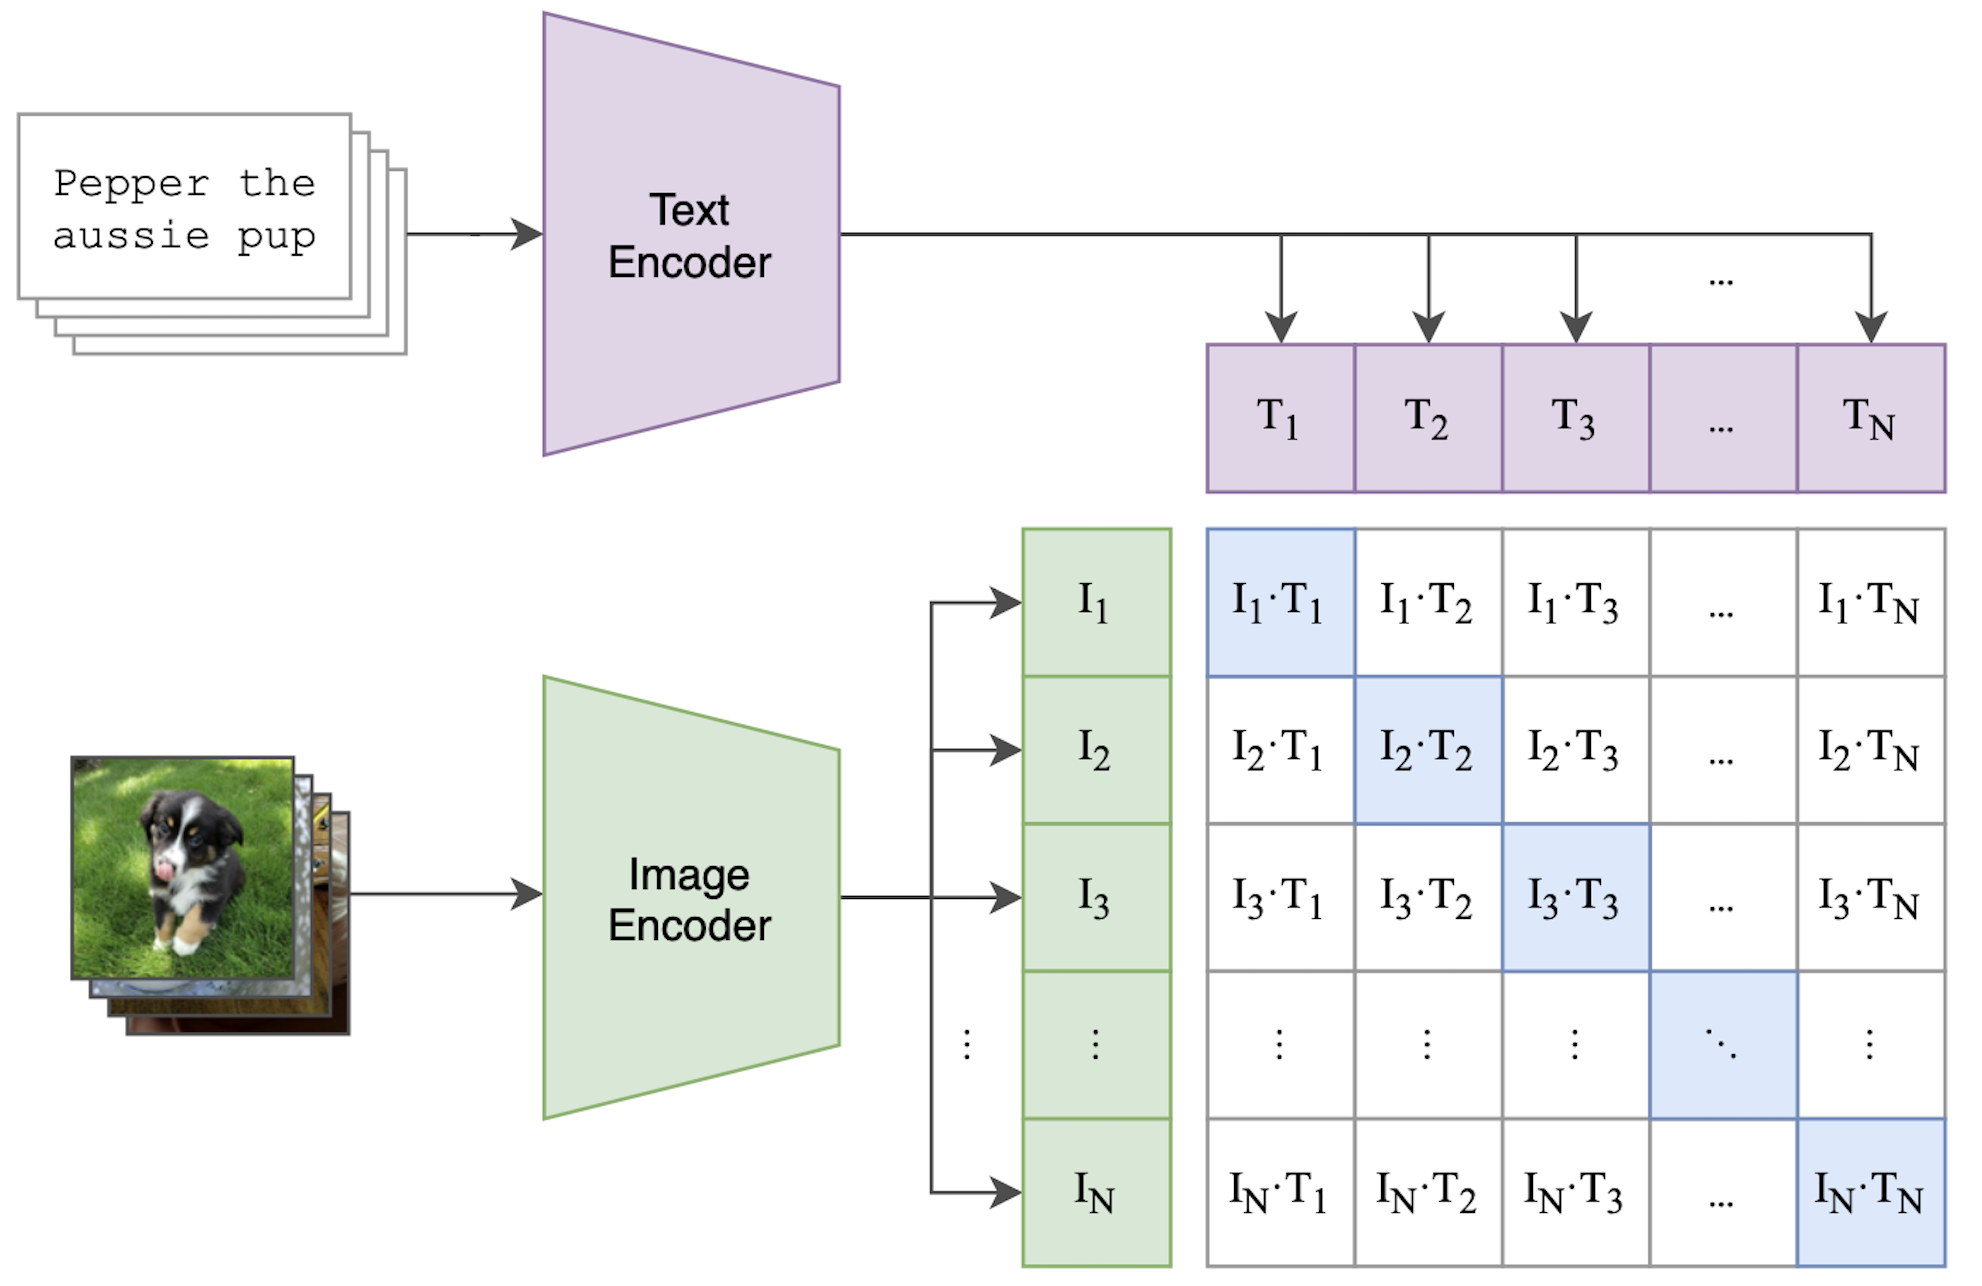
\includegraphics[width=0.7\textwidth]{CLIP_architecture_small}
                \end{figure}
            \end{column}
        \end{columns}
    \end{onlyenv}

    \begin{onlyenv}<4>
        \begin{equation*}
            \operatorname{L_{InfoNCE}} =
            - \frac{1}{N} \ln \sum_{i=1}^{N} \frac{\exp(\textcolor{Rhodamine}{\tau}^{-1} \mathbf{x}_i^T \mathbf{y}_i)}{\sum_{j=1}^{N} \exp(\textcolor{Rhodamine}{\tau}^{-1} \mathbf{x}_i^T \mathbf{y}_j)}
            - \frac{1}{N} \sum_{i=1}^{N} \ln \frac{\exp(\textcolor{Rhodamine}{\tau}^{-1} \mathbf{x}_i^T \mathbf{y}_i)}{\sum_{j=1}^{N} \exp(\textcolor{Rhodamine}{\tau}^{-1} \mathbf{x}_j^T \mathbf{y}_i)}
        \end{equation*}
        \begin{columns}
            \begin{column}{0.5\textwidth}
                \begin{itemize}
                    \item $\mathbf{x}_i$ --- image embedding
                    \item $\mathbf{y}_i$ --- text embedding
                    \item \textcolor{Rhodamine}{$\tau$} --- temperature, inverse entropy
                \end{itemize}
            \end{column}
            \begin{column}{0.5\textwidth}
                \begin{figure}
                    \centering
                    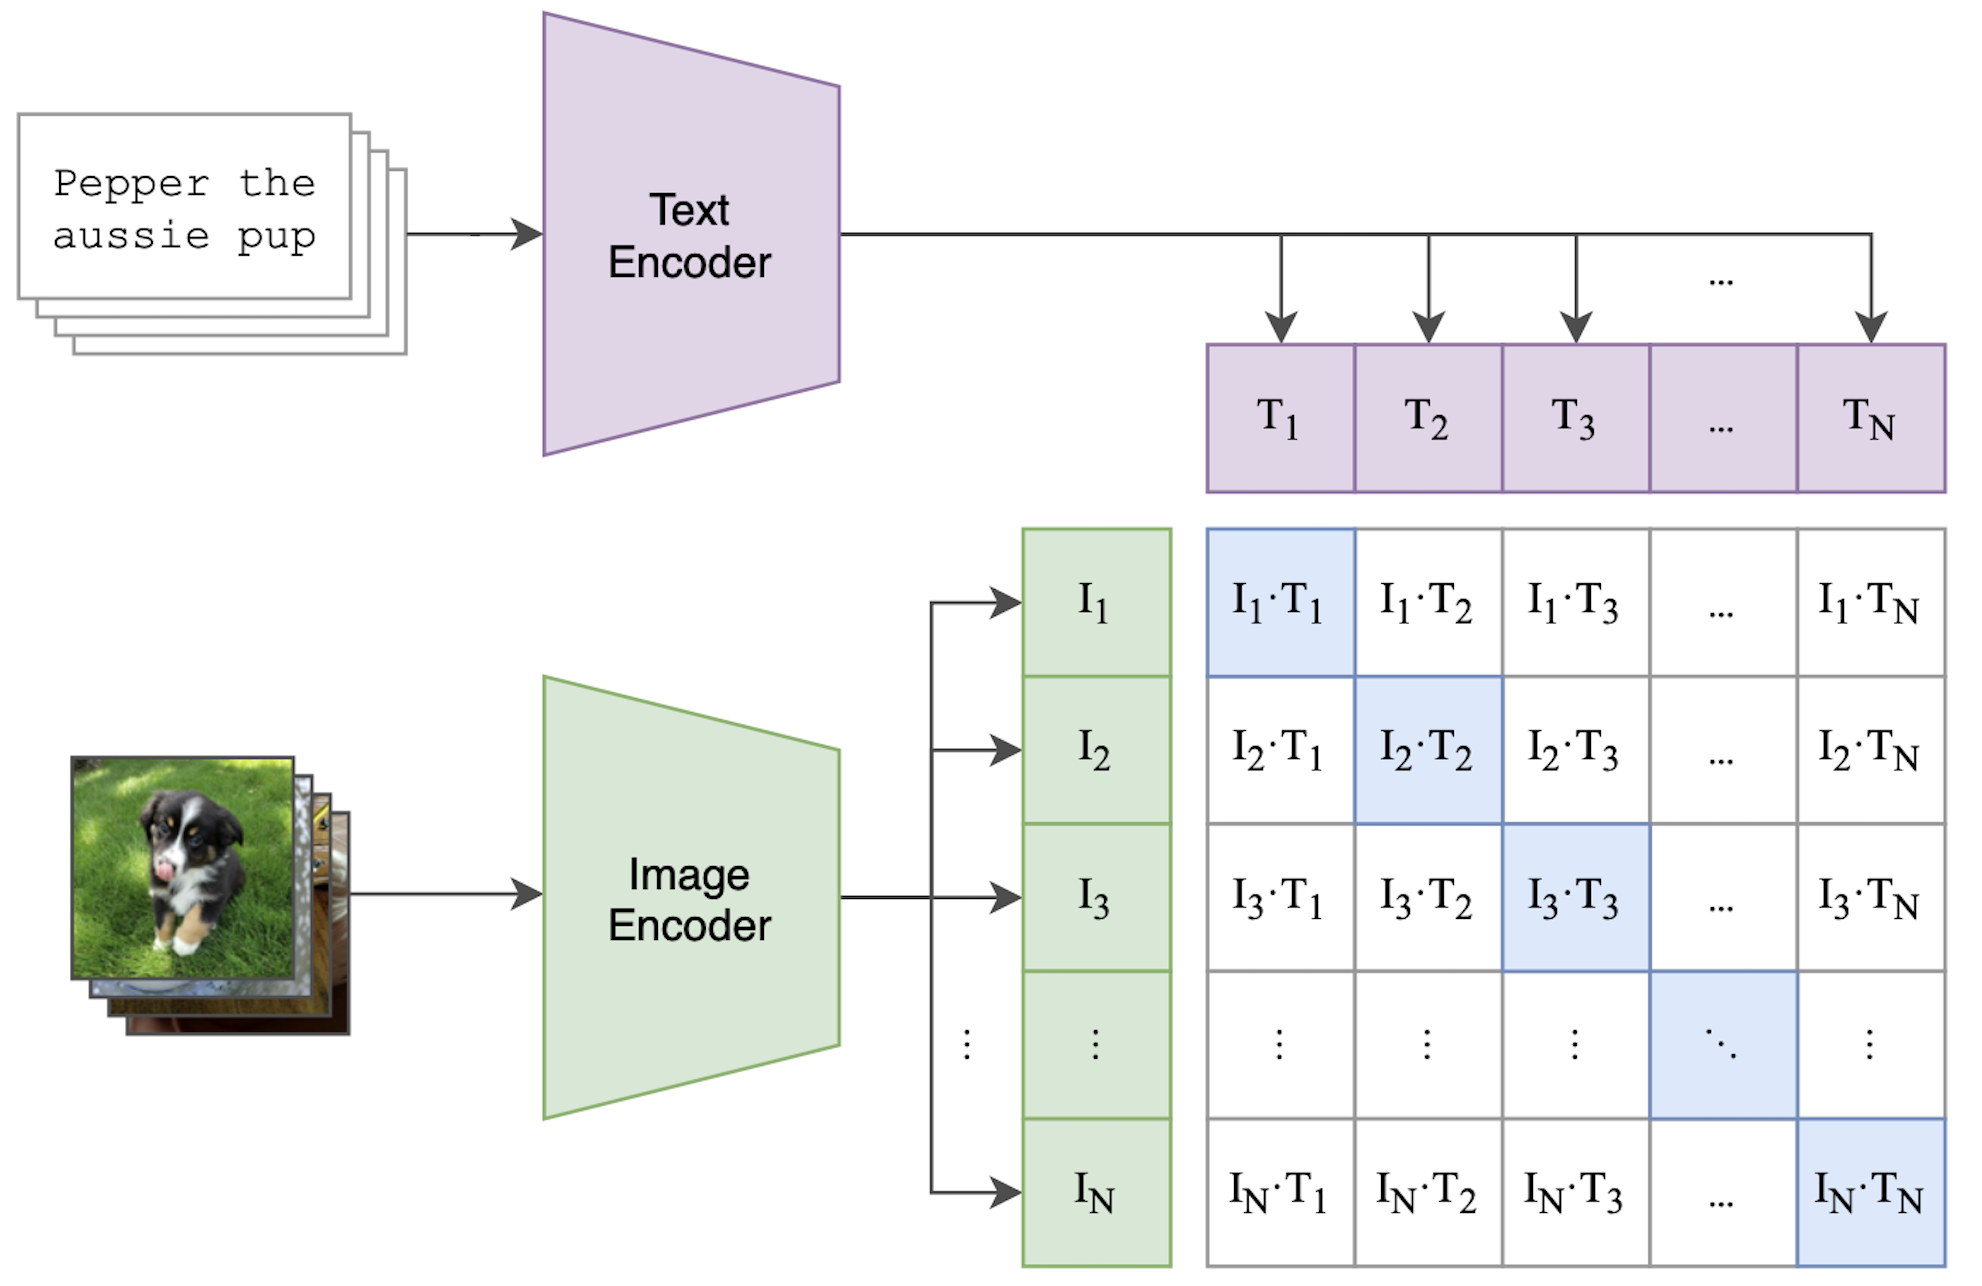
\includegraphics[width=0.7\textwidth]{CLIP_architecture_small}
                \end{figure}
            \end{column}
        \end{columns}
    \end{onlyenv}

    \begin{onlyenv}<5>
        \begin{equation*}
            \operatorname{L_{InfoNCE}} =
            - \frac{1}{N} \ln \sum_{i=1}^{N} \frac{\exp(\tau^{-1} \mathbf{x}_i^T \mathbf{y}_i)}{\sum_{j=1}^{N} \exp(\tau^{-1} \mathbf{x}_i^T \mathbf{y}_j)}
            - \frac{1}{N} \sum_{i=1}^{N} \ln \frac{\exp(\tau^{-1} \mathbf{x}_i^T \mathbf{y}_i)}{\sum_{j=1}^{N} \exp(\tau^{-1} \mathbf{x}_j^T \mathbf{y}_i)}
        \end{equation*}
        \begin{columns}
            \begin{column}{0.5\textwidth}
                \begin{itemize}
                    \item $\mathbf{x}_i$ --- image embedding
                    \item $\mathbf{y}_i$ --- text embedding
                    \item $\tau$ --- temperature, inverse entropy
                    \item $\Vert \mathbf{x}_i \Vert = \Vert \mathbf{y}_j \Vert = 1 \ \Rightarrow \ \cos(\mathbf{x}_i, \mathbf{y}_j) = \mathbf{x}_i^T \mathbf{y}_j$
                \end{itemize}
            \end{column}
            \begin{column}{0.5\textwidth}
                \begin{figure}
                    \centering
                    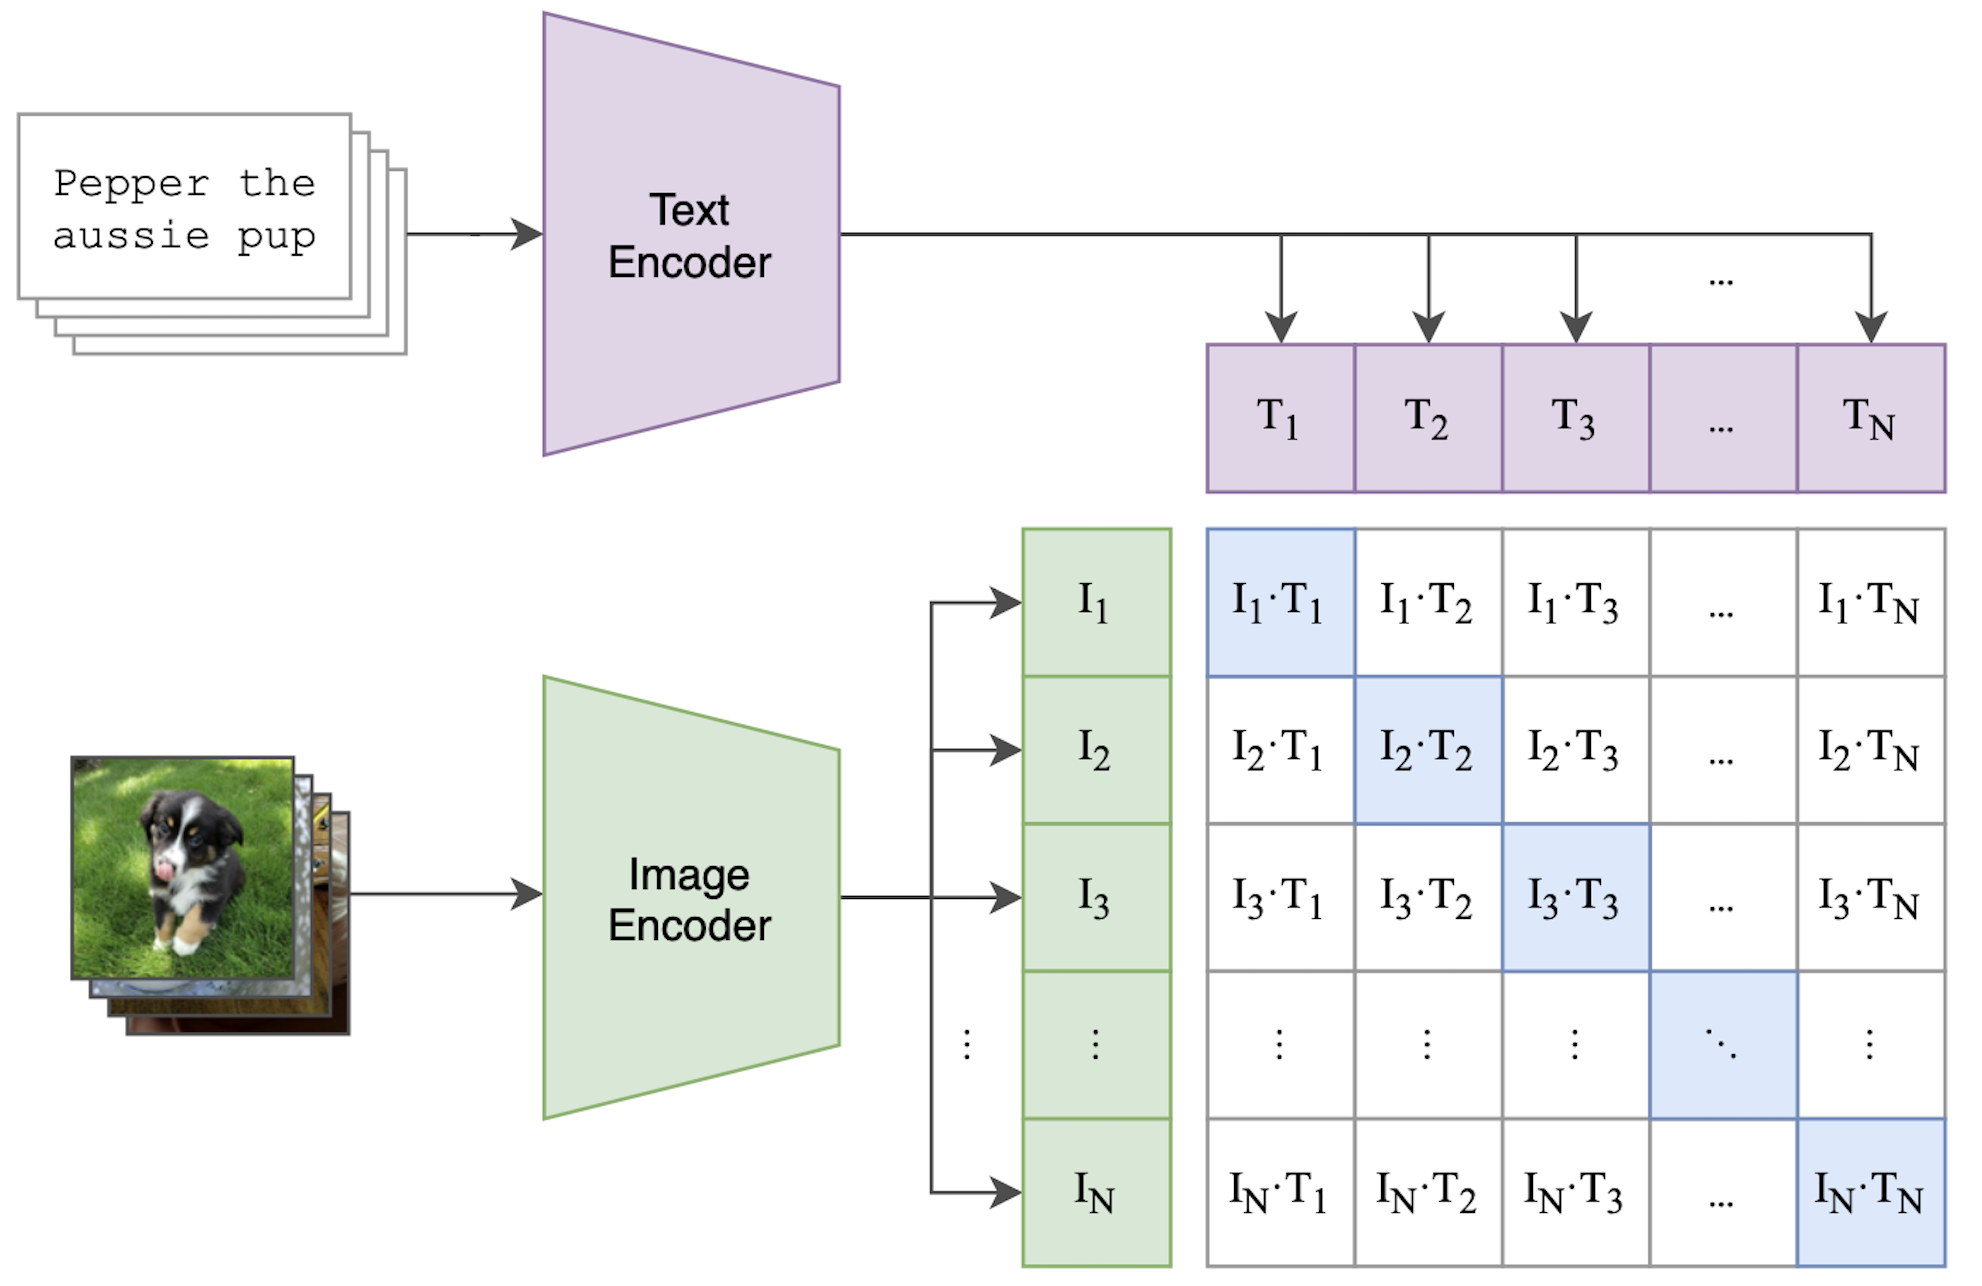
\includegraphics[width=0.7\textwidth]{CLIP_architecture_small}
                \end{figure}
            \end{column}
        \end{columns}
    \end{onlyenv}
\end{frame}

\begin{frame}[t]{InfoLOOB (Leave One Out Bound) --- CLOOB's Objective}
    \small%
    \begin{onlyenv}<1>
        \centering%
        \begin{equation*}
            \operatorname{L_{InfoLOOB}} =
            - \frac{1}{N} \ln \sum_{i=1}^{N} \frac{\exp(\tau^{-1} \mathbf{x}_i^T \mathbf{y}_i)}{\sum_{\textcolor{red}{j \neq i}}^{N} \exp(\tau^{-1} \mathbf{x}_i^T \mathbf{y}_j)}
            - \frac{1}{N} \sum_{i=1}^{N} \ln \frac{\exp(\tau^{-1} \mathbf{x}_i^T \mathbf{y}_i)}{\sum_{\textcolor{red}{j \neq i}}^{N} \exp(\tau^{-1} \mathbf{x}_j^T \mathbf{y}_i)}
        \end{equation*}
    \end{onlyenv}
    \begin{onlyenv}<2->
        \footnotesize%
        \centering%
        \begin{equation*}
            \operatorname{L_{InfoLOOB}} =
            - \frac{1}{N} \ln \sum_{i=1}^{N} \frac{\exp(\tau^{-1} \mathbf{x}_i^T \mathbf{y}_i)}{\sum_{j \neq i}^{N} \exp(\tau^{-1} \mathbf{x}_i^T \mathbf{y}_j)}
            - \frac{1}{N} \sum_{i=1}^{N} \ln \frac{\exp(\tau^{-1} \mathbf{x}_i^T \mathbf{y}_i)}{\sum_{j \neq i}^{N} \exp(\tau^{-1} \mathbf{x}_j^T \mathbf{y}_i)}
        \end{equation*}
    \end{onlyenv}
    \footnotesize
    \action<2->{
    \begin{equation*}
        \operatorname{L_{InfoNCE}}(\mathbf{y}_1) =
        - \ln \frac{\overbrace{\exp(\tau^{-1} \mathbf{x}_1^T \mathbf{y}_1)}^{\textcolor{Cyan}{a}}}{\underbrace{\exp(\tau^{-1} \mathbf{x}_1^T \mathbf{y}_1)}_{\textcolor{Cyan}{a}} + \underbrace{\textstyle\sum_{j=2}^{N} \exp(\tau^{-1} \mathbf{x}_j^T \mathbf{y}_1)}_{\textcolor{Magenta}{b}}}
    \end{equation*}}
    \action<3->{
    \begin{tikzpicture}[frameoverlay]
        \path
         (0.75,0.373) node{\textcolor{red}{\larr  \textbf{saturation problem}}};
     \end{tikzpicture}}
    \action<4->{
    \begin{equation*}
        \operatorname{L_{InfoLOOB}}(\mathbf{y}_1) =
        - \ln \frac{\overbrace{\exp(\tau^{-1} \mathbf{x}_1^T \mathbf{y}_1)}^{\textcolor{Cyan}{a}}}{\underbrace{\textstyle\sum_{j=2}^{N} \exp(\tau^{-1} \mathbf{x}_j^T \mathbf{y}_1)}_{\textcolor{Magenta}{b}}}
    \end{equation*}}
\end{frame}

\begin{frame}[fragile]{CLOOB (Contrastive Leave One Out Boost)}
    \noindent
    \hspace*{\fill}%
    \begin{minipage}{0.8\textwidth}
        \centering

        \begin{onlyenv}<1>
            \begin{multicols}{2}
                \begin{lstlisting}[language=Python, basicstyle=\tiny]


















 \end{lstlisting}
                \columnbreak
                \begin{lstlisting}[language=Python, basicstyle=\tiny, firstnumber=last]

















 \end{lstlisting}
            \end{multicols}
        \end{onlyenv}

        \begin{onlyenv}<2>
            \begin{multicols}{2}
                \begin{lstlisting}[language=Python, basicstyle=\tiny]
# image_encoder - ResNet
# text_encoder - Text Transformer

# I[n, h, w, c] - minibatch of images
# T[n, l] - minibatch of texts

# W_i[d_i, d_e] - image projection
# W_t[d_t, d_e] - text projection

# beta - inverse temperature Hopfield retrieval
# tau - temperature InfoLOOB







 \end{lstlisting}
                \columnbreak
                \begin{lstlisting}[language=Python, basicstyle=\tiny, firstnumber=last]

















 \end{lstlisting}
            \end{multicols}
        \end{onlyenv}

        \begin{onlyenv}<3>
            \begin{multicols}{2}
                \begin{lstlisting}[language=Python, basicstyle=\tiny]
# image_encoder - ResNet
# text_encoder - Text Transformer

# I[n, h, w, c] - minibatch of images
# T[n, l] - minibatch of texts

# W_i[d_i, d_e] - image projection
# W_t[d_t, d_e] - text projection

# beta - inverse temperature Hopfield retrieval
# tau - temperature InfoLOOB

# extract feature representations
I_f = image_encoder(I) #[n, d_i]
T_f = text_encoder(T) #[n, d_t]



 \end{lstlisting}
                \columnbreak
                \begin{lstlisting}[language=Python, basicstyle=\tiny, firstnumber=last]

















 \end{lstlisting}
            \end{multicols}
        \end{onlyenv}

        \begin{onlyenv}<4>
            \begin{multicols}{2}
                \begin{lstlisting}[language=Python, basicstyle=\tiny]
# image_encoder - ResNet
# text_encoder - Text Transformer

# I[n, h, w, c] - minibatch of images
# T[n, l] - minibatch of texts

# W_i[d_i, d_e] - image projection
# W_t[d_t, d_e] - text projection

# beta - inverse temperature Hopfield retrieval
# tau - temperature InfoLOOB

# extract feature representations
I_f = image_encoder(I) #[n, d_i]
T_f = text_encoder(T) #[n, d_t]

# joint multimodal embedding
x = l2_normalize(I_f @ W_i) #[n, d_e]
y = l2_normalize(T_f @ W_t) #[n, d_e]\end{lstlisting}
                \columnbreak
                \begin{lstlisting}[language=Python, basicstyle=\tiny, firstnumber=last]

















 \end{lstlisting}
            \end{multicols}
        \end{onlyenv}

        \begin{onlyenv}<5>
            \begin{multicols}{2}
                \begin{lstlisting}[language=Python, basicstyle=\tiny]
# image_encoder - ResNet
# text_encoder - Text Transformer

# I[n, h, w, c] - minibatch of images
# T[n, l] - minibatch of texts

# W_i[d_i, d_e] - image projection
# W_t[d_t, d_e] - text projection

# beta - inverse temperature Hopfield retrieval
# tau - temperature InfoLOOB

# extract feature representations
I_f = image_encoder(I) #[n, d_i]
T_f = text_encoder(T) #[n, d_t]

# joint multimodal embedding
x = l2_normalize(I_f @ W_i) #[n, d_e]
y = l2_normalize(T_f @ W_t) #[n, d_e]\end{lstlisting}
                \columnbreak
                \begin{lstlisting}[language=Python, basicstyle=\tiny, firstnumber=last]
# Hopfield retrieval H with batch stored
# H(beta, A, B) = B.T @ softmax(beta * A @ B.T)
U_x = H(beta, x, x).T #[n, d_e]
U_y = H(beta, y, x).T #[n, d_e]
V_x = H(beta, x, y).T #[n, d_e]
V_y = H(beta, y, y).T #[n, d_e]











 \end{lstlisting}
            \end{multicols}
        \end{onlyenv}

        \begin{onlyenv}<6>
            \begin{multicols}{2}
                \begin{lstlisting}[language=Python, basicstyle=\tiny]
# image_encoder - ResNet
# text_encoder - Text Transformer

# I[n, h, w, c] - minibatch of images
# T[n, l] - minibatch of texts

# W_i[d_i, d_e] - image projection
# W_t[d_t, d_e] - text projection

# beta - inverse temperature Hopfield retrieval
# tau - temperature InfoLOOB

# extract feature representations
I_f = image_encoder(I) #[n, d_i]
T_f = text_encoder(T) #[n, d_t]

# joint multimodal embedding
x = l2_normalize(I_f @ W_i) #[n, d_e]
y = l2_normalize(T_f @ W_t) #[n, d_e]\end{lstlisting}
                \columnbreak
                \begin{lstlisting}[language=Python, basicstyle=\tiny, firstnumber=last]
# Hopfield retrieval H with batch stored
# H(beta, A, B) = B.T @ softmax(beta * A @ B.T)
U_x = H(beta, x, x).T #[n, d_e]
U_y = H(beta, y, x).T #[n, d_e]
V_x = H(beta, x, y).T #[n, d_e]
V_y = H(beta, y, y).T #[n, d_e]

# normalize retrievals
U_x = l2_normalize(U_x) #[n, d_e] 
U_y = l2_normalize(U_y) #[n, d_e] 
V_x = l2_normalize(V_x) #[n, d_e] 
V_y = l2_normalize(V_y) #[n, d_e]





 \end{lstlisting}
            \end{multicols}
        \end{onlyenv}

        \begin{onlyenv}<7>
            \begin{multicols}{2}
                \begin{lstlisting}[language=Python, basicstyle=\tiny]
# image_encoder - ResNet
# text_encoder - Text Transformer

# I[n, h, w, c] - minibatch of images
# T[n, l] - minibatch of texts

# W_i[d_i, d_e] - image projection
# W_t[d_t, d_e] - text projection

# beta - inverse temperature Hopfield retrieval
# tau - temperature InfoLOOB

# extract feature representations
I_f = image_encoder(I) #[n, d_i]
T_f = text_encoder(T) #[n, d_t]

# joint multimodal embedding
x = l2_normalize(I_f @ W_i) #[n, d_e]
y = l2_normalize(T_f @ W_t) #[n, d_e]\end{lstlisting}
                \columnbreak
                \begin{lstlisting}[language=Python, basicstyle=\tiny, firstnumber=last]
# Hopfield retrieval H with batch stored
# H(beta, A, B) = B.T @ softmax(beta * A @ B.T)
U_x = H(beta, x, x).T #[n, d_e]
U_y = H(beta, y, x).T #[n, d_e]
V_x = H(beta, x, y).T #[n, d_e]
V_y = H(beta, y, y).T #[n, d_e]

# normalize retrievals
U_x = l2_normalize(U_x) #[n, d_e] 
U_y = l2_normalize(U_y) #[n, d_e] 
V_x = l2_normalize(V_x) #[n, d_e] 
V_y = l2_normalize(V_y) #[n, d_e]

# loss: info_loob(tau, anchors, samples) 
# samples contain pos. and neg. embeddings 
loss_i = info_loob(tau, U_x, U_y)
loss_t = info_loob(tau, V_y, V_x)
loss = (loss_i + loss_t) * tau\end{lstlisting}
            \end{multicols}
        \end{onlyenv}
    \end{minipage}
    \hspace*{\fill}
\end{frame}

%%%%%%%%%%%%%%%%%%%%%%%%%%%%%%%%%%%%%%%%%%%%%%%%%%%%%%%%%%%%%%%%%%%%%%%%%%%%%%%%%%%%%%%%%%%%%%%%%%%%%
\section{Experiments}

\begin{frame}{Experiments}
    \pause
    \begin{itemize}
        \item Conceptual Captions (CC) Pretraining
        \begin{itemize}
            \item rich textual description
            \item only 2.9 million images
        \end{itemize}
        \pause
        \item Yahoo Flickr Create Commons (YFCC) Pretraining
        \begin{itemize}
            \item less rich textual description
            \item 15 million images
        \end{itemize}
        \pause
        \item Both tested on seven image classification datasets
        \pause
        \item Ablation studies
        \begin{itemize}
            \item Modern Hopfield networks
            \item InfoLOOB
        \end{itemize}
    \end{itemize}
\end{frame}

\begin{frame}{CLIP and CLOOB: Results}
    \begin{columns}
        \begin{column}{0.5\textwidth}
            \begin{table}
                \centering
                \caption*{CC --- mean accuracy over 5 runs}
                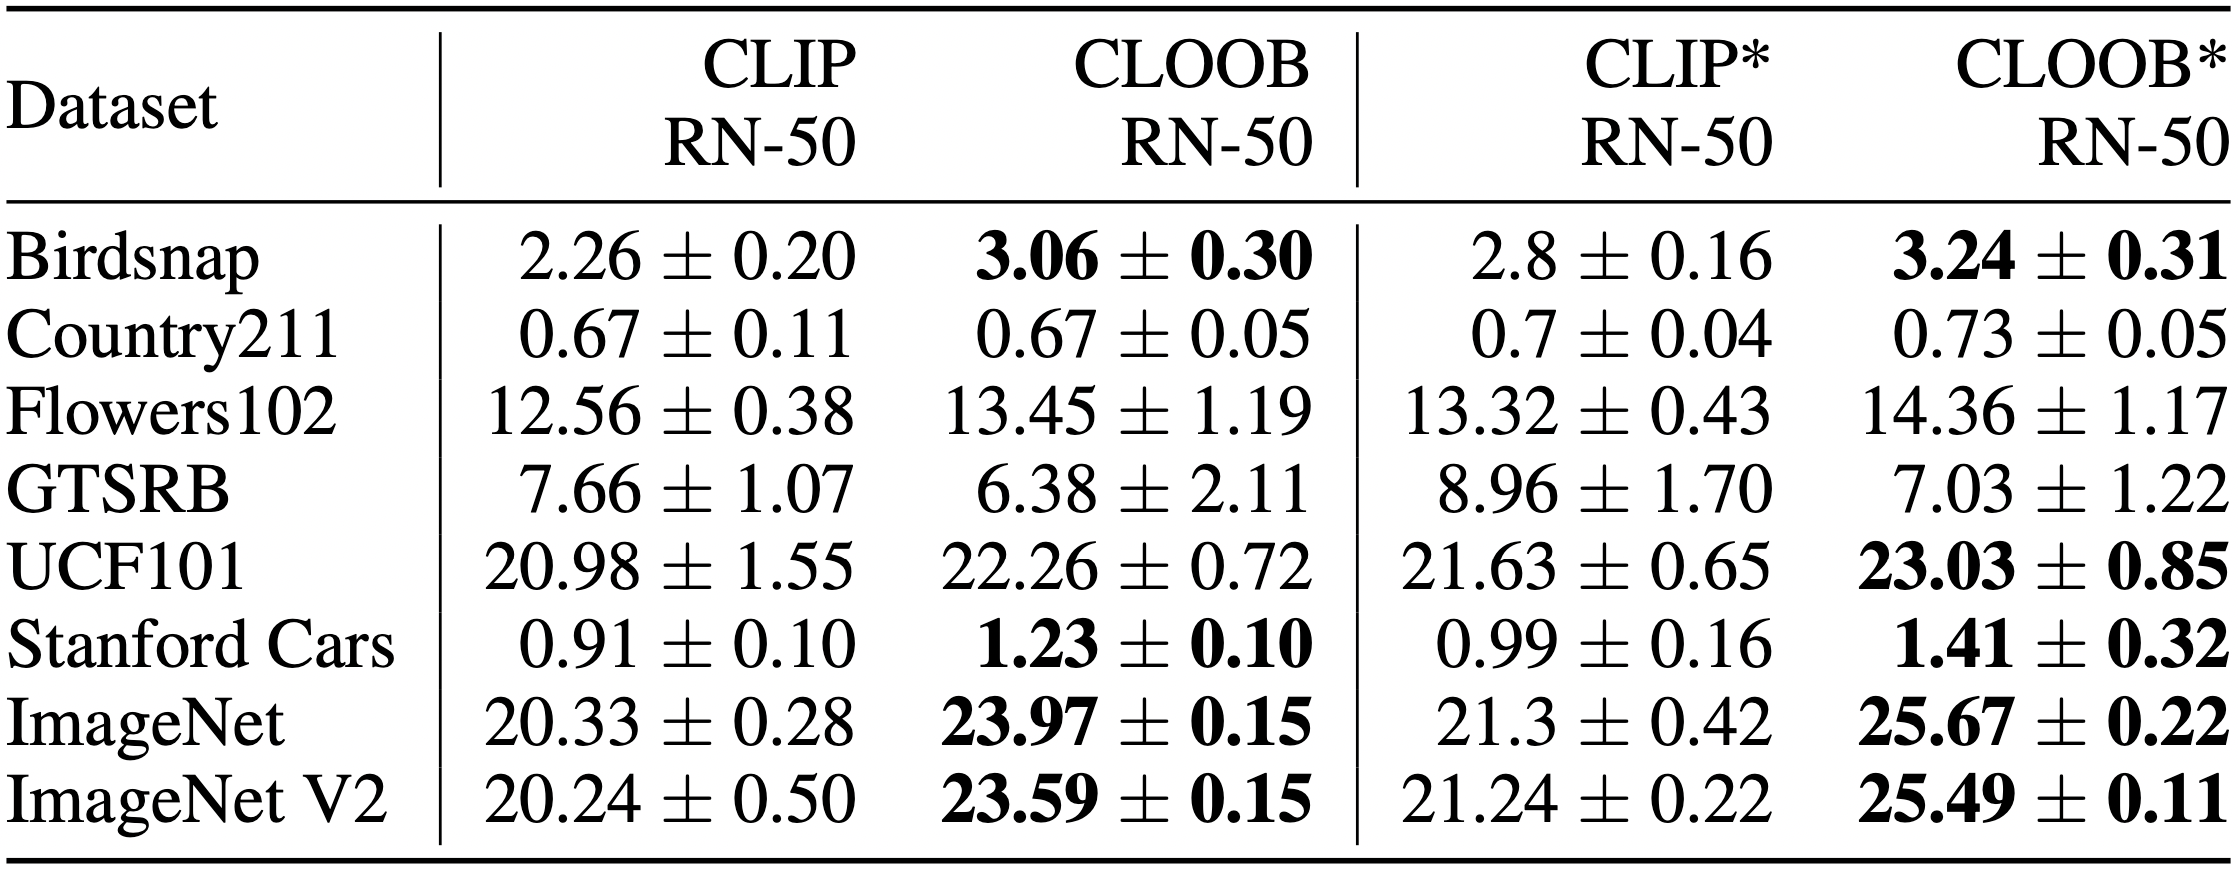
\includegraphics[width=0.9\textwidth]{cc_table}
            \end{table}
            \centering
            Bold: statistically significant
        \end{column}
        \begin{column}{0.5\textwidth}
            \begin{table}
                \centering
                \caption*{YFCC --- one run}
                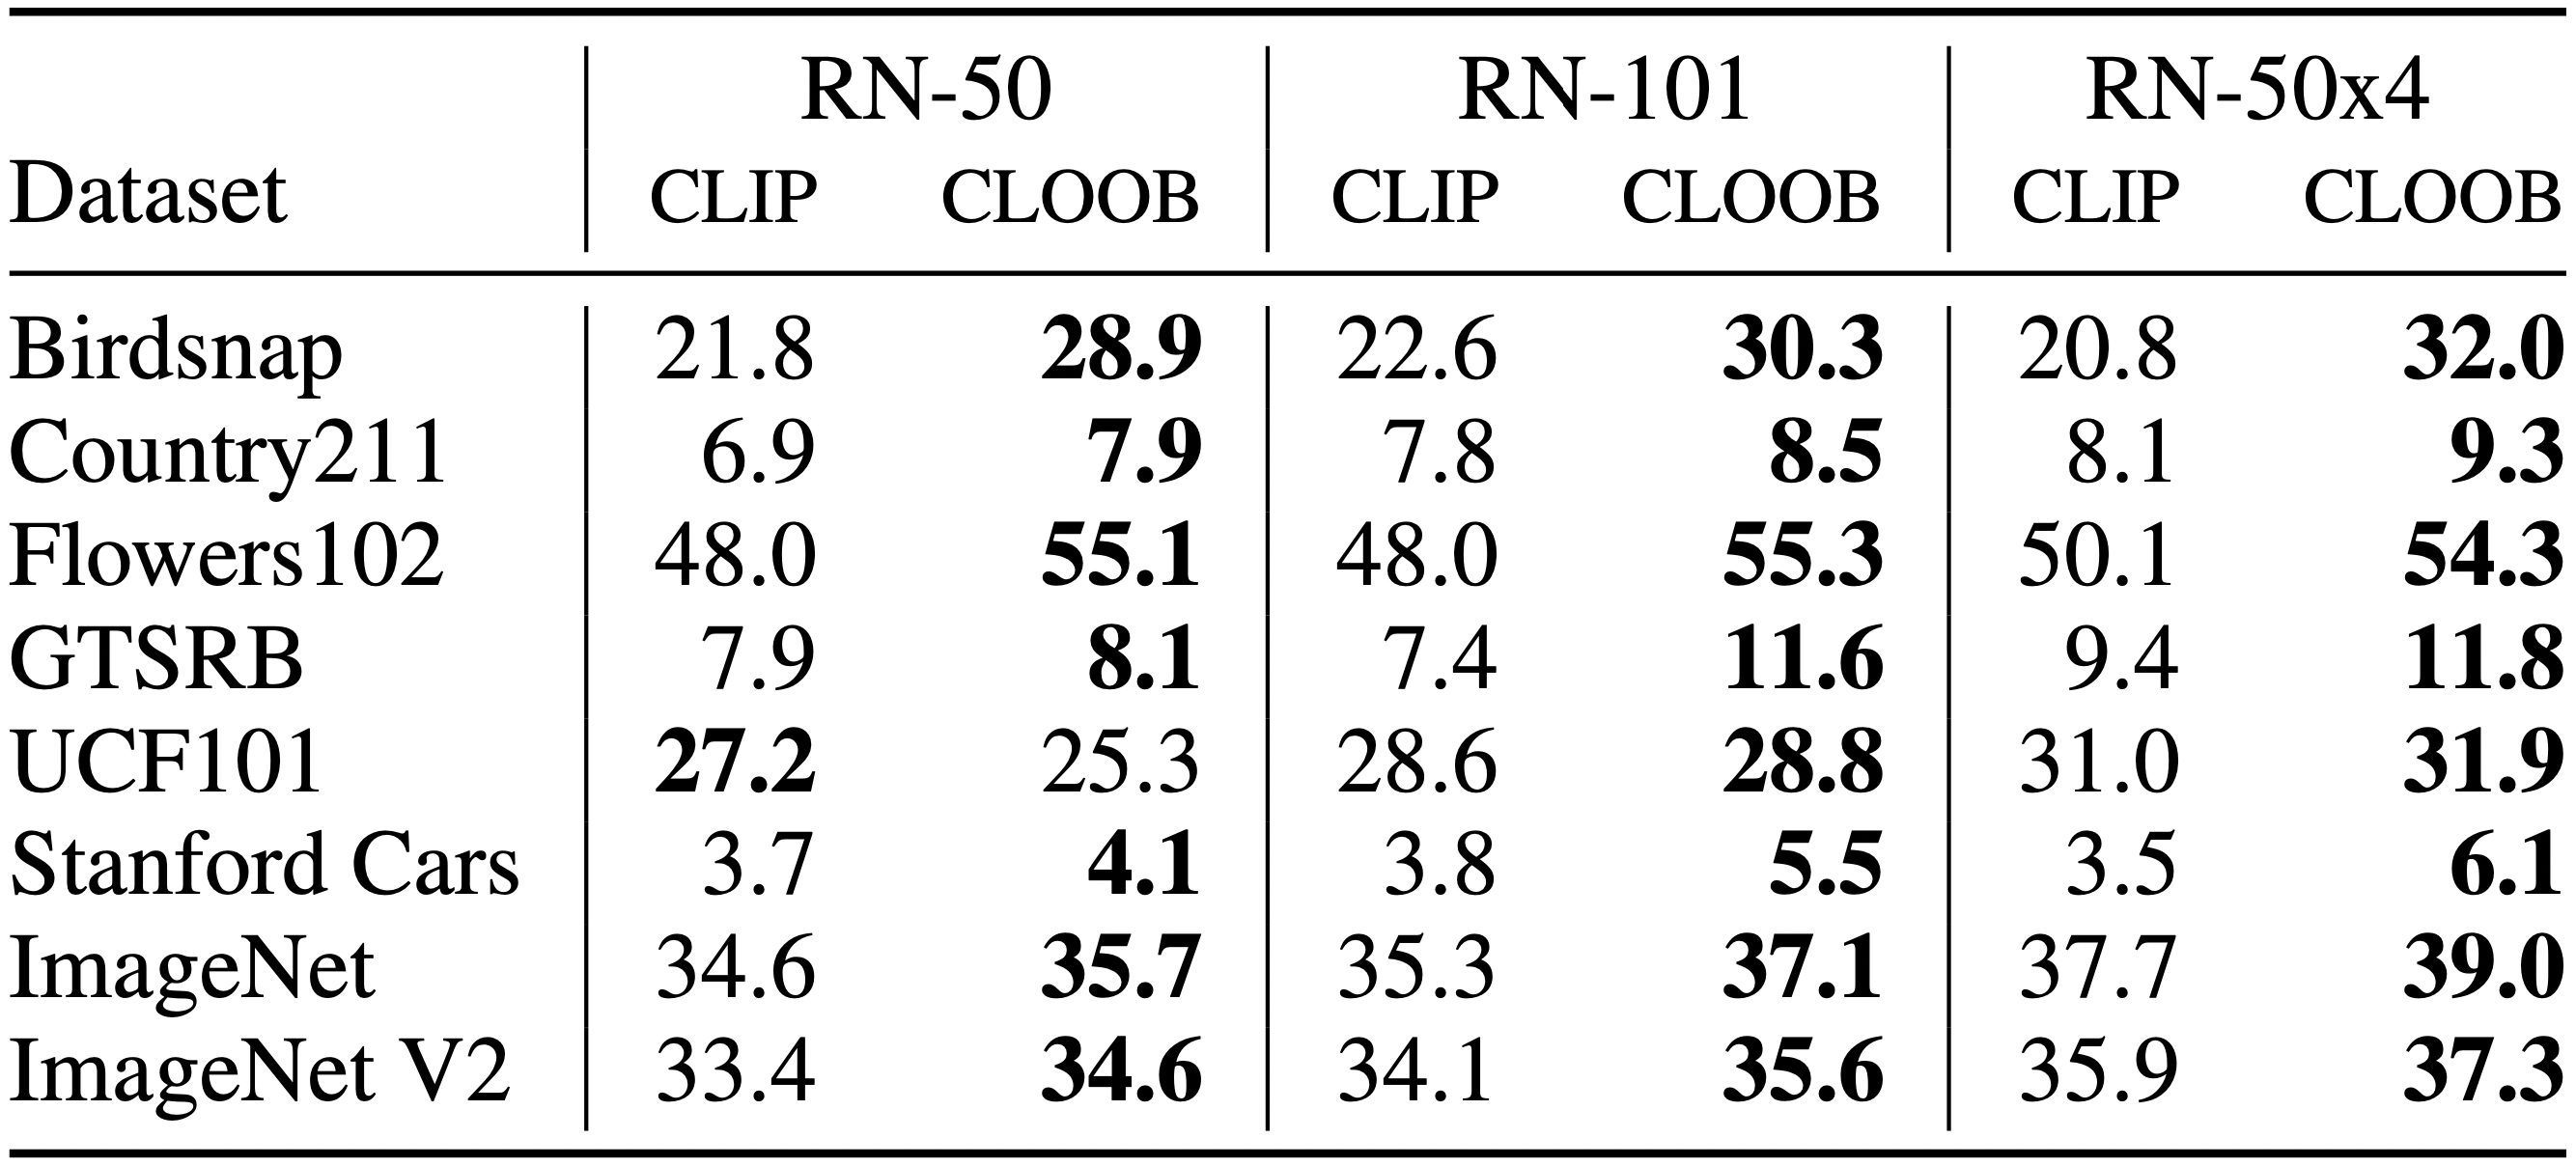
\includegraphics[width=0.9\textwidth]{yfcc_table}
            \end{table}
            \centering
            Bold: higher value
        \end{column}
    \end{columns}
\end{frame}

\begin{frame}{Results Ablation Study}
    \vspace*{\fill} 
    \begin{figure}
        \centering
        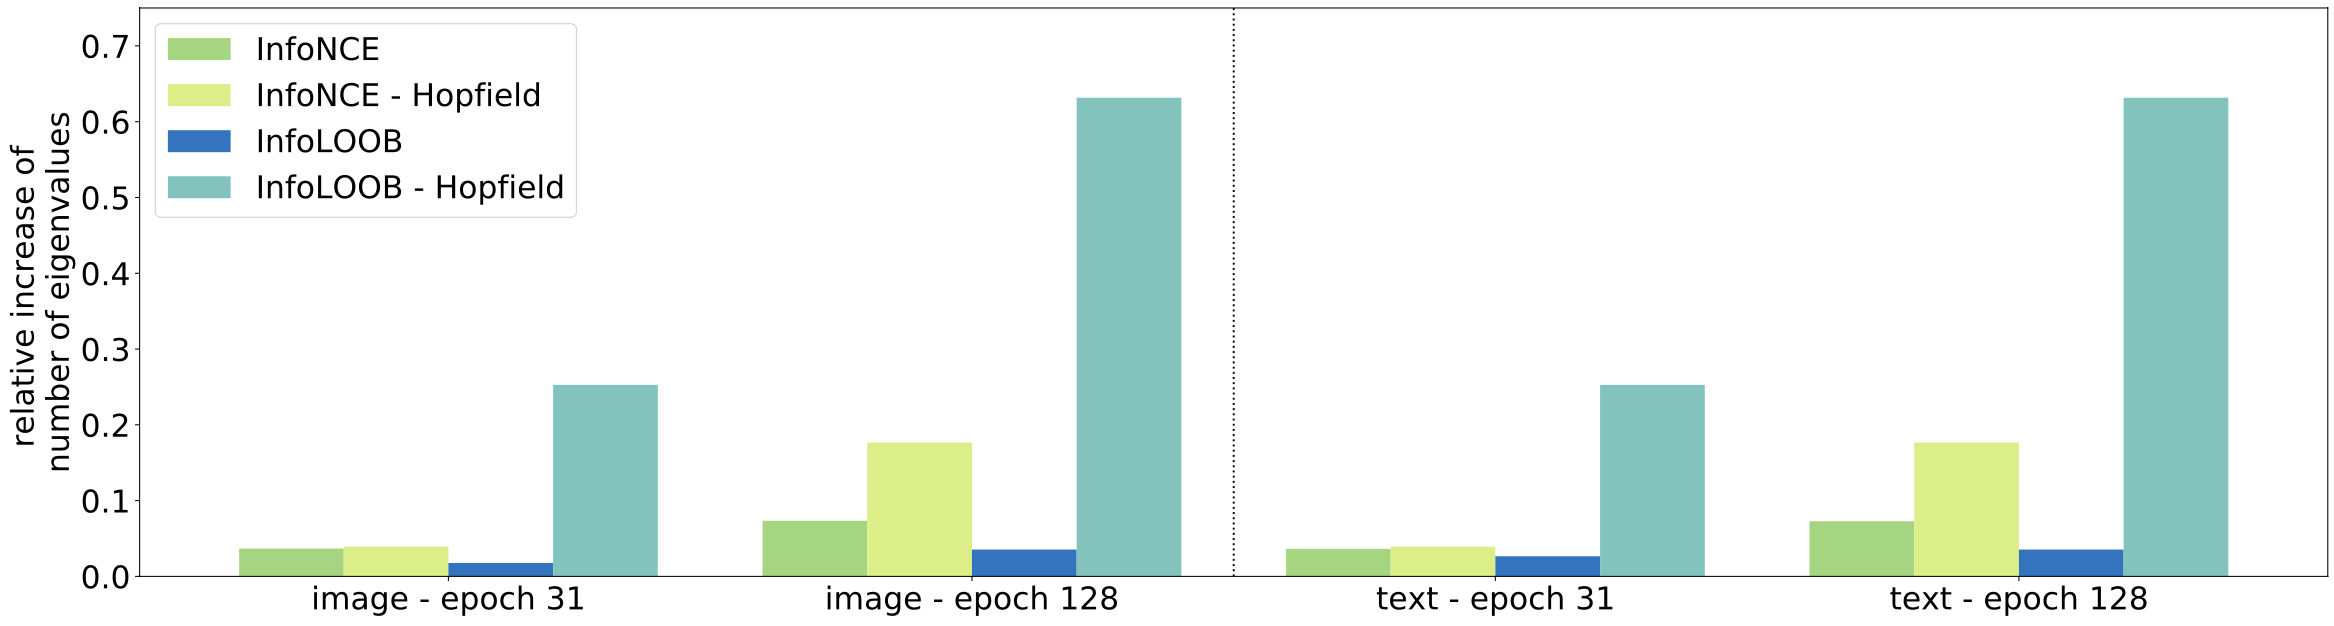
\includegraphics[width=1.0\textwidth]{eigenvalues}
    \end{figure}
    \vspace*{\fill}
\end{frame}

%%%%%%%%%%%%%%%%%%%%%%%%%%%%%%%%%%%%%%%%%%%%%%%%%%%%%%%%%%%%%%%%%%%%%%%%%%%%%%%%%%%%%%%%%%%%%%%%%%%%%
\section{Conclusion}

\begin{frame}{Critical Assessment}
    \pause
    \begin{itemize}
        \item Reproducibility
        \begin{itemize}
            \item hyperparameters, experiments well-defined \cmark
            \item code, datasets public \cmark
        \end{itemize}
        \pause
        \item Thoroughness
        \begin{itemize}
            \item two theorems, both proven \cmark
            \item all assumptions listed \cmark
        \end{itemize}
        \pause
        \item Fairness of comparison
        \begin{itemize}
            \item as faithful to original CLIP as possible \cmark
            \item CLIP's 400 million image dataset not public
        \end{itemize}
    \end{itemize}
    \pause
    Paper fulfills all NeurIPS check marks
\end{frame}

\begin{frame}{Summary}
    \begin{columns}
        \begin{column}{0.4\textwidth}
            \begin{itemize}
                \item[\rarr] CLIP \pause
                \begin{itemize}
                    \item[\xmark] explaining away \pause
                \end{itemize}
                \item[\rarr] Modern Hopfield networks \pause
                \begin{itemize}
                    \item[\xmark] saturation problem \pause
                \end{itemize}
                \item[\rarr] CLOOB \pause
                \begin{itemize}
                    \item[\cmark] Modern Hopfield networks \pause
                    \item[\cmark] InfoLOOB \pause
                \end{itemize}
                \item[\rarr] \smiley{} \pause
            \end{itemize}
        \end{column}
        \begin{column}{0.6\textwidth}
            \begin{figure}
                \centering
                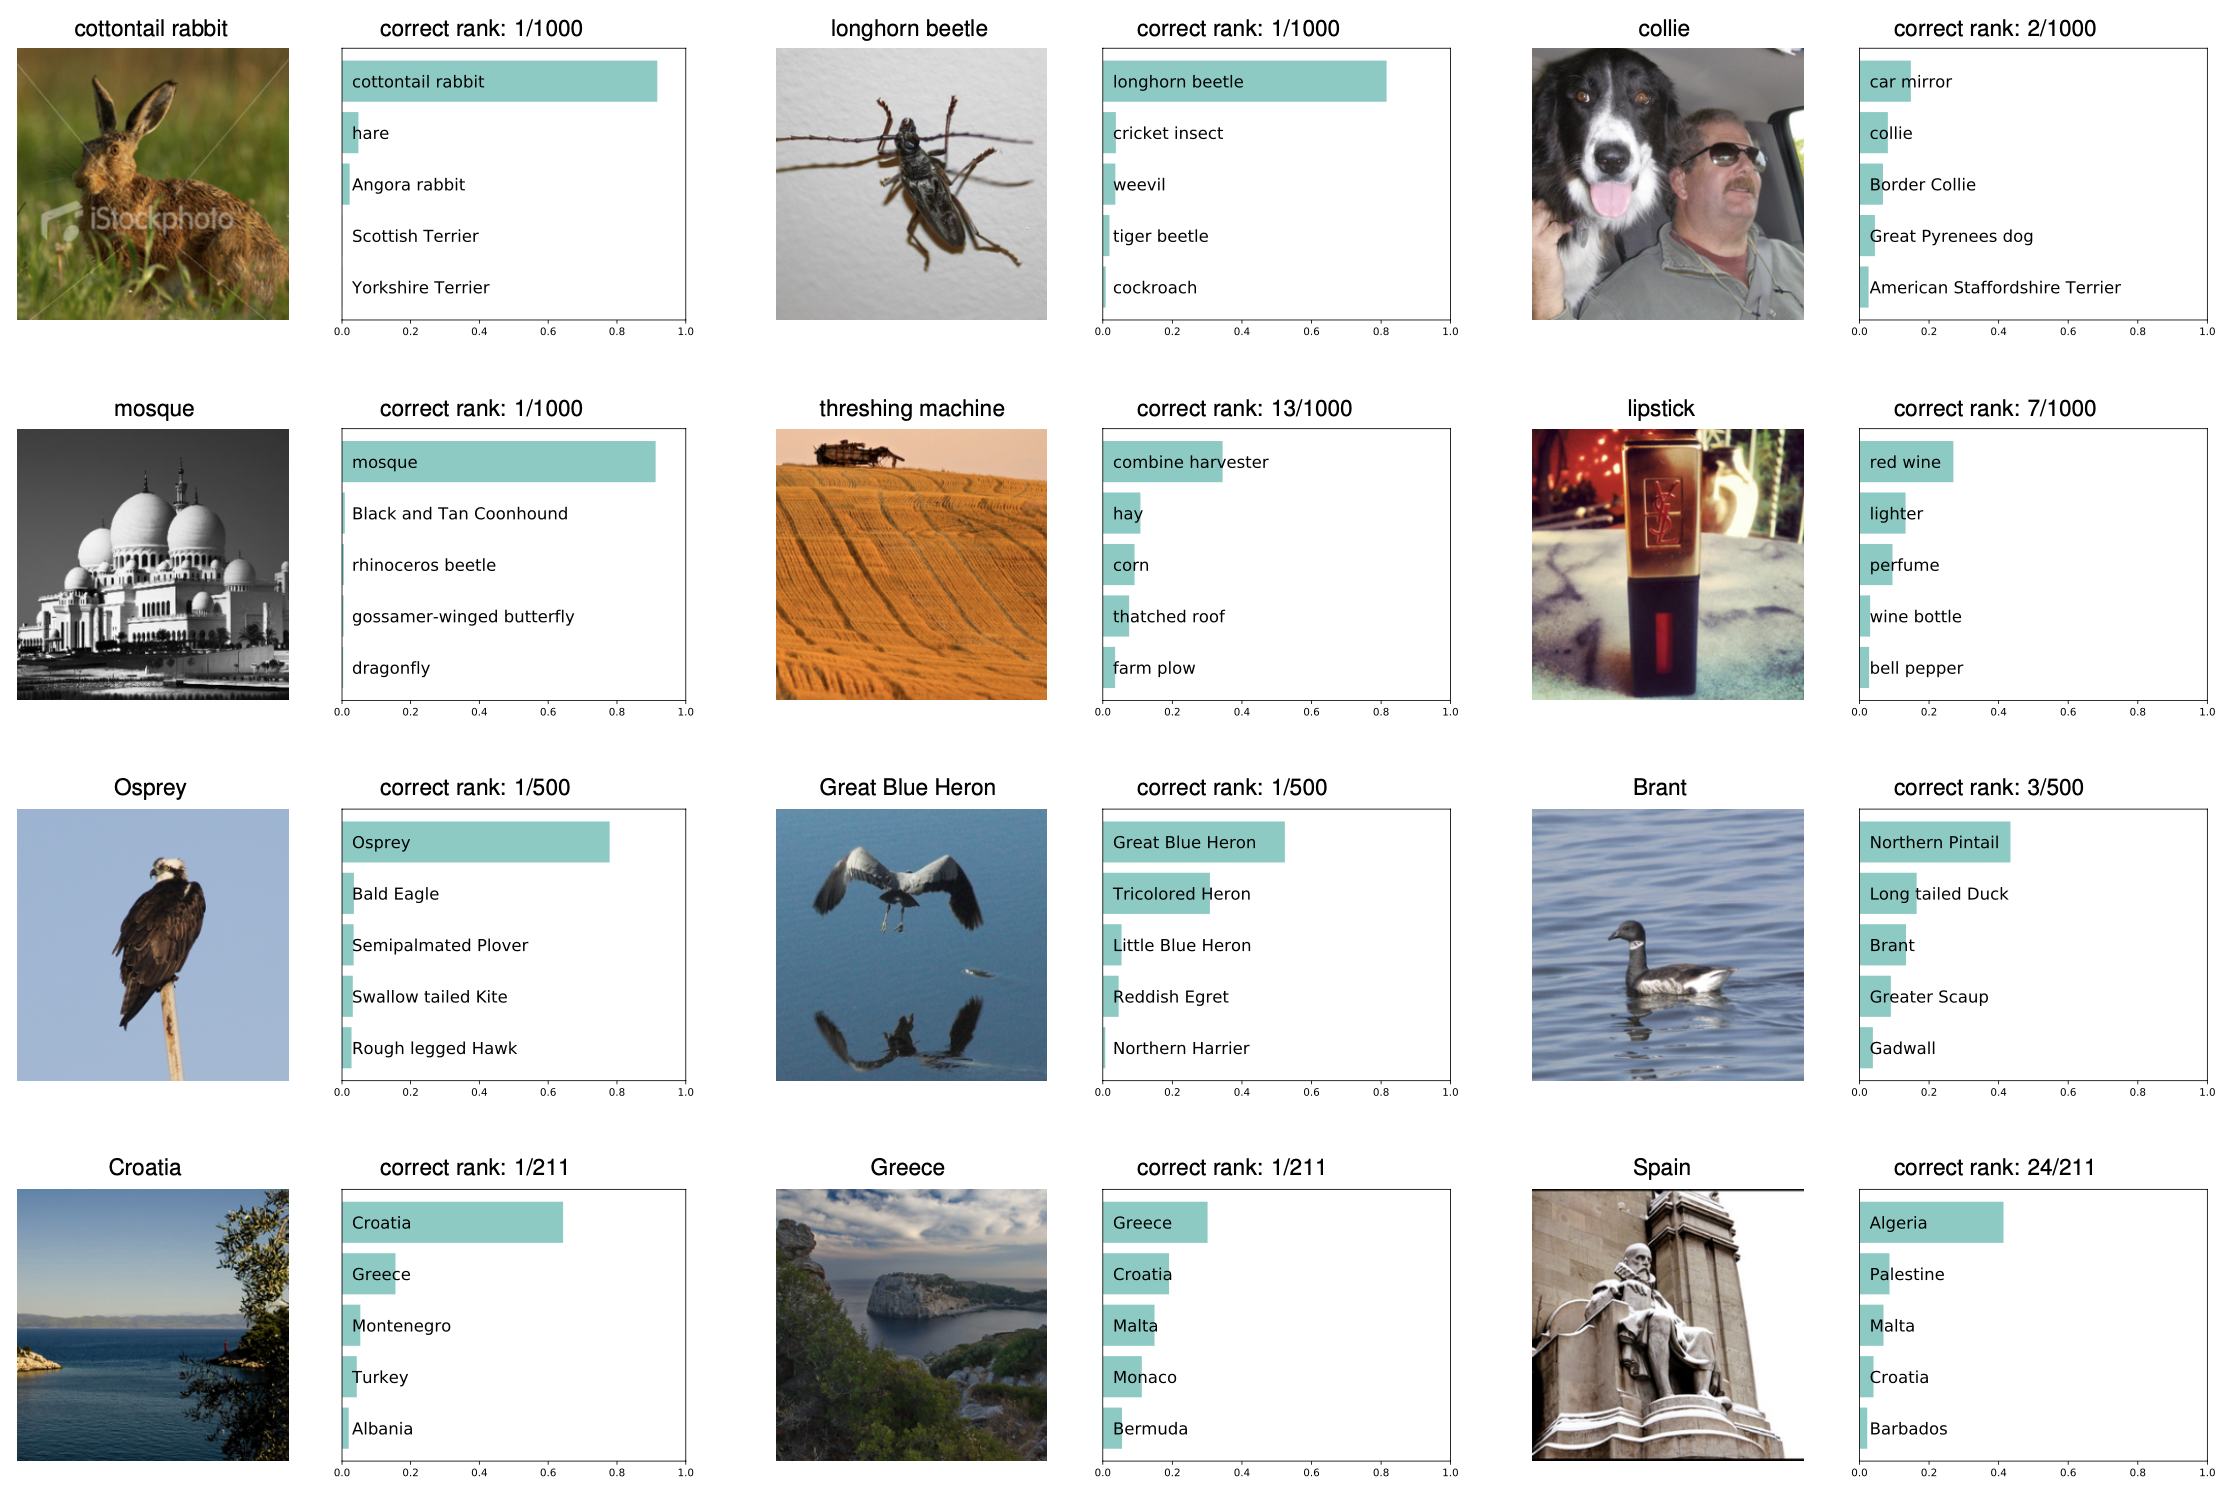
\includegraphics[width=0.9\textwidth]{zero_shot}
            \end{figure}
        \end{column}
    \end{columns}
\end{frame}

%%%%%%%%%%%%%%%%%%%%%%%%%%%%%%%%%%%%%%%%%%%%%%%%%%%%%%%%%%%%%%%%%%%%%%%%%%%%%%%%%%%%%%%%%%%%%%%%%%%%%
\section{Additional Material}

\begin{frame}{Distribution of Cosine Similarity}
    \vspace*{\fill} 
    \begin{figure}
        \centering
        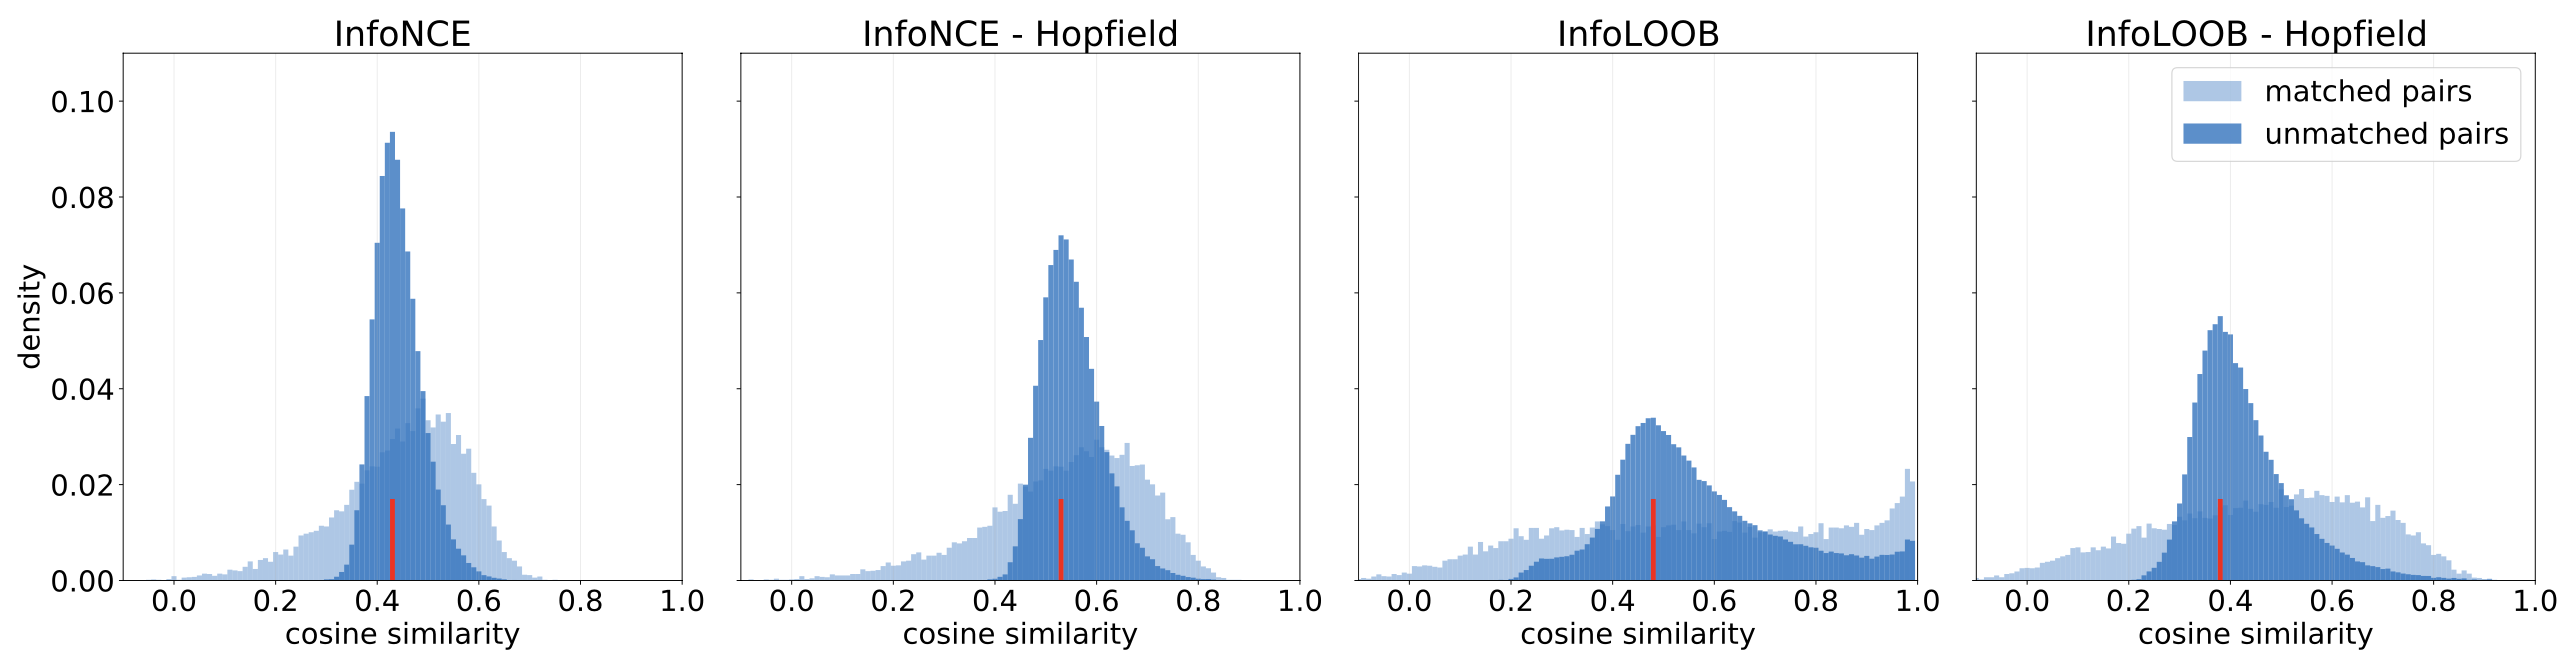
\includegraphics[width=1.0\textwidth]{ablation}
        \caption*{Distribution of cosine similarity of matched pairs and of the 10 unmatched pairs that have the highest similarity score with anchor}
    \end{figure}
    \vspace*{\fill} 
\end{frame}

\begin{frame}{Ajne Test}
    \begin{figure}
        \centering
        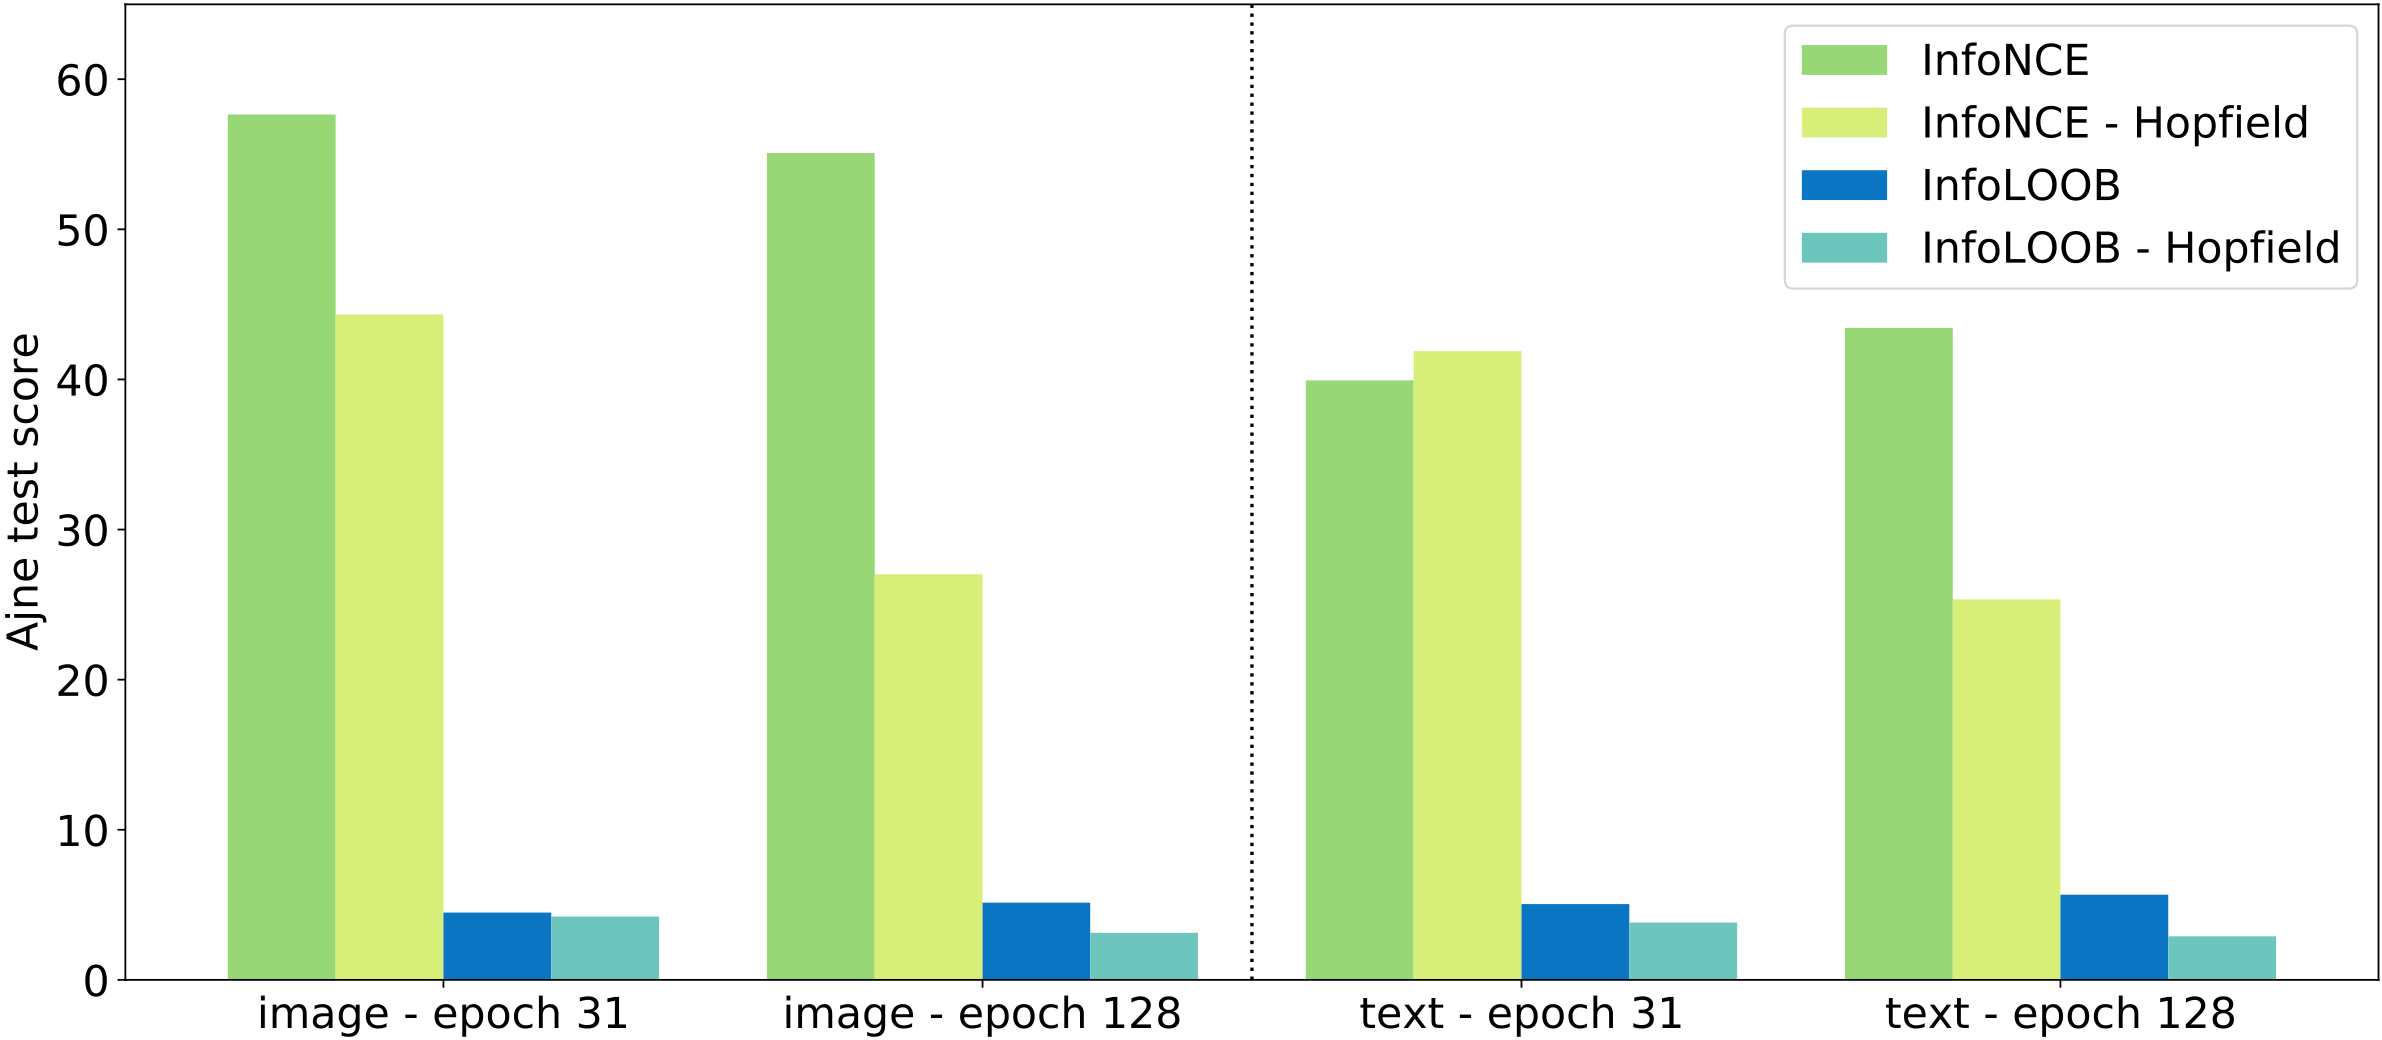
\includegraphics[width=0.8\textwidth]{Ajne}
    \end{figure}
\end{frame}

\begin{frame}{InfoLOOB -- Further details}
    \hspace*{\fill}%
    \begin{tblr}{ |c||c|c| }
        \hline
         &$\mathbf{\textcolor{red}{u}}_i$ - stored \textcolor{red}{image} emb.&$\mathbf{\textcolor{blue}{v}}_i$ - stored \textcolor{blue}{text} emb.\\
         \hline\hline
         $\mathbf{\textcolor{red}{x}}_i$ - \textcolor{red}{image} query emb.&$\mathbf{\textcolor{red}{U}}_{\mathbf{\textcolor{red}{x}}_i}$ - \textcolor{red}{image}-retr. \textcolor{red}{image} emb.&$\mathbf{\textcolor{blue}{V}}_{\mathbf{\textcolor{red}{x}}_i}$ - \textcolor{red}{image}-retr. \textcolor{blue}{text} emb.\\
         \hline
         $\mathbf{\textcolor{blue}{y}}_i$ - \textcolor{blue}{text} query emb.&$\mathbf{\textcolor{red}{U}}_{\mathbf{\textcolor{blue}{y}}_i}$ - \textcolor{blue}{text}-retr. \textcolor{red}{image} emb.&$\mathbf{\textcolor{blue}{V}}_{\mathbf{\textcolor{blue}{y}}_i}$ - \textcolor{blue}{text}-retr. \textcolor{blue}{text} emb.\\
        \hline
    \end{tblr}
    \hspace*{\fill}%
    \begin{equation*}
        \operatorname{L_{InfoLOOB}} =
        - \frac{1}{N} \ln \sum_{i=1}^{N} \frac{\exp(\tau^{-1} \mathbf{\textcolor{red}{U}}_{\mathbf{\textcolor{red}{x}}_i}^T \mathbf{\textcolor{red}{U}}_{\mathbf{\textcolor{blue}{y}}_i})}{\sum_{j \neq i}^{N} \exp(\tau^{-1} \mathbf{\textcolor{red}{U}}_{\mathbf{\textcolor{red}{x}}_i}^T \mathbf{\textcolor{red}{U}}_{\mathbf{\textcolor{blue}{y}}_j})}
        - \frac{1}{N} \sum_{i=1}^{N} \ln \frac{\exp(\tau^{-1} \mathbf{\textcolor{blue}{V}}_{\mathbf{\textcolor{red}{x}}_i}^T \mathbf{\textcolor{blue}{V}}_{\mathbf{\textcolor{blue}{y}}_i})}{\sum_{j \neq i}^{N} \exp(\tau^{-1} \mathbf{\textcolor{blue}{V}}_{\mathbf{\textcolor{red}{x}}_j}^T \mathbf{\textcolor{blue}{V}}_{\mathbf{\textcolor{blue}{y}}_i})}
    \end{equation*}
    \hspace*{\fill}%
\end{frame}

\begin{frame}{Gradients of InfoLOOB and InfoNCE}
    \footnotesize
    \begin{equation*}
        \frac{\partial}{\partial \mathbf{y}} \operatorname{L_{InfoNCE}}(\mathbf{y})
        = \frac{\partial}{\partial \mathbf{y}} - \ln \frac{\exp(\tau^{-1} \mathbf{x}_1^T \mathbf{y}_1)}{\textstyle\sum_{j=1}^{N} \exp(\tau^{-1} \mathbf{x}_j^T \mathbf{y})}
        = - \tau^{-1} \mathbf{y}^T \mathbf{x}_1 + \tau^{-1} \operatorname{lse}(\tau^{-1}, \mathbf{X}^T \mathbf{y})
    \end{equation*}
    \begin{equation*}
        \frac{\partial}{\partial \mathbf{y}} \operatorname{L_{InfoLOOB}}(\mathbf{y})
        = \frac{\partial}{\partial \mathbf{y}} - \ln \frac{\exp(\tau^{-1} \mathbf{x}_1^T \mathbf{y}_1)}{\textstyle\sum_{j \neq i}^{N} \exp(\tau^{-1} \mathbf{x}_j^T \mathbf{y})}
        = - \tau^{-1} \mathbf{y}^T \mathbf{x}_1 + \tau^{-1} \operatorname{lse}(\tau^{-1}, \tilde{\mathbf{X}}^T \mathbf{y})
    \end{equation*}
    \begin{equation*}
        \frac{\partial}{\partial \mathbf{y}} \operatorname{L_{InfoNCE}}(\mathbf{y})
        = - \tau^{-1} (1 - p_1) (\mathbf{x}_1 - \tilde{\mathbf{X}} \operatorname{softmax}(\tau^{-1} \tilde{\mathbf{X}}^T \mathbf{y}))
        = (1-p_1) \frac{\partial}{\partial \mathbf{y}} \operatorname{L_{InfoLOOB}}(\mathbf{y})
    \end{equation*}
    \begin{equation*}
        \operatorname{lse}(\beta, \boldsymbol{\alpha}) = \beta^{-1} \log \left( \sum_{i=1}^{N}\exp(\beta \alpha_i) \right)
    \end{equation*}
    \begin{equation*}
        \mathbf{X} = (\mathbf{x}_1, \dots, \mathbf{x}_N), \quad \tilde{\mathbf{X}} = (\mathbf{x}_2, \dots, \mathbf{x}_N)
    \end{equation*}
\end{frame}

\addtocounter{framenumber}{-5}
\end{document}